%############################# Anhang #################################
\appendix
%\chapter{Mathematischer Anhang}
%\chapter{Programmcodes}
\chapter{Appendix}

Write here small introduction to appendix! %TODO
\clearpage
\section{Complete Feature List}

The geometrical features have shortened names, but everything in capital letters, refer to the container
dimensions. For example, W,L and H refer to the width, length and height of the container. Consecutively,
WLH is the multiplication of all container dimensions and displays the maximum container volume.

\begin{table}[ht]
    \centering
    \small
    \renewcommand{\arraystretch}{1.3}
    \begin{tabular}{@{}cccc@{}}
        NoCustomers            & width-height-min   & width-W-min   & volume-WLH-min   \\
        NoItems                & width-height-max   & width-W-max   & volume-WLH-max   \\
        Rel Volume             & width-height-mean  & width-W-mean  & volume-WLH-mean  \\
        Rel Weight             & width-height-std   & width-W-std   & volume-WLH-std   \\
        Rel Total Length Items & length-height-min  & length-L-min  & height-area-min  \\
        Rel Total Width Items  & length-height-max  & length-L-max  & height-area-max  \\
        Rel Total Height Items & length-height-mean & length-L-mean & height-area-mean \\
        Fragile Ratio          & length-height-std  & length-L-std  & height-area-std  \\
        Fragile Sequence       & width-length-min   & height-H-min  & area-AREA-min    \\
        Volume Balance         & width-length-max   & height-H-max  & area-AREA-max    \\
        Volume Distribution    & width-length-mean  & height-H-mean & area-AREA-mean   \\
        Weight Distribution    & width-length-std   & height-H-std  & area-AREA-std    \\
    \end{tabular}
    \caption{Complete feature list.}
    \label{tab:complete_features_list}
\end{table}

\clearpage
\section{Random Route Generation}
\label{chap:appendix:RRG}
This appendix chapter helps understanding the algorithm used for the generation of random routes. The complete algorithm
is depicted in Figure~\ref{fig:flowchart_randomRouteGeneration} and the following Algorithm~\ref{alg:appendix:check_single_tour}
is used to check the volume and weight limit of one single tour.
\begin{algorithm}[ht]
    \caption{Check volume and weight limit}
    \label{alg:appendix:check_single_tour}
    \begin{algorithmic}[1]\onehalfspacing
        \Require{Volume limit $V$, Weight limit $Q$, Uniform distribution $\mathcal{U}(a,b)$}
        \Procedure{Feasible}{$\text{Route}\,R,\, \text{Lower Threshold}\,\delta$}
        \State{Get subset of customers $S$ from route $R$}
        \State{$V^* \gets V \cdot \mathcal{U}(\delta,\,1)$} \Comment{Individual bounds for each single route}
        \State{$Q^* \gets Q \cdot \mathcal{U}(\delta,\,1)$}
        \If{$q(S)\le Q^* \, \wedge \, v(S)\le V^*$} \Comment{Check feasibility}
        \State{\textbf{return} true}
        \Else
        \State{\textbf{return} false}
        \EndIf
        \EndProcedure
    \end{algorithmic}
\end{algorithm}

As the following flowchart contains a lot of information and many different symbols the used terms are explained in
the following. The parameters $\mathcal{I}$, $\alpha$, $\beta$, $\gamma$ and $\delta$ were alredady described in
Section~\ref{sec:DataRetrieval}.

\begin{itemize}\singlespacing
    \item $\mathcal{G}$: Set of found routes
    \item $i$: Current instance
    \item $n$: Numbers of customers / Length of route
    \item $n_{max}$: Maximum numbers of customers in instance $i$
    \item $c$: Counter for inner loops finding no tour
    \item $t$: Iteration counter for inner loop (no function!)
    \item $k$: Counter for found tours in the inner loop
    \item $a$: Counter for failed attempts to find a feasible tour
    \item $x$: Counter for breakups
    \item SuccessBool: Boolean, if at least one route was found in inner loop
    \item BreakBool: Boolean for interrupting current instance $i$, when for one customer number $n$ no route could be found
\end{itemize}



\begin{figure}[ht]
    \centering
    \footnotesize
    \begin{tikzpicture}[
            scale = 0.983, transform shape,node distance=7mm and 11mm,
            >=Latex,
            % Styles
            startstop/.style   = {rectangle, draw, align=center, minimum width=22mm, minimum height=6mm},
            process/.style     = {rectangle, draw, align=center, minimum width=30mm, minimum height=6mm},
            decision/.style    = {diamond, draw, aspect=2, inner sep=1pt, align=center, minimum width=40mm,minimum height=20mm},
            io/.style          = {trapezium, trapezium left angle=60, trapezium right angle=120, draw, align=center, minimum height=6mm},
            connector/.style   = {circle, draw, inner sep=1pt},
            line/.style        = {->}
        ]

        % Nodes
        \node[startstop] (start) {Start RRG ($\mathcal{I}$, $\alpha$, $\beta$, $\gamma$, $\delta$)};
        \node[decision, below=of start] (forI) {$i\in\mathcal{I}$ left?};
        \node[process, left= of forI] (nextI) {Next $i$ \&\\ Save $\mathcal{G}$};
        \node[process, below=of forI] (initI) {$\mathcal{G}\gets\emptyset$\\$n_{\max}\gets \mathrm{MaxCustomers}(i)$\\BreakBool$\gets$False};
        \node[decision, below=5mm of initI] (forN) {$n=2\ \to\ n_{\max}$ left?};
        \node[decision, below=of forN] (exitOuter) {BreakBool?};
        \node[decision, right=of exitOuter] (breakDec) {$c \geq n \cdot \alpha$?};
        \node[startstop] at ($(breakDec.north |- forI.east)$) (end) {End RRG};
        \node[decision, below=of exitOuter] (forAlpha) {$t=1\ \to\ n\cdot\alpha$ left?};
        \node[decision, below=of forAlpha] (whileK) {While\\$k<\gamma$?};
        \node[decision, below=12 mm of whileK] (dup) {$R\in\mathcal{G}$?};
        % \node[process, bel=of dup] (drawThresh) {$Q^*\gets Q\cdot \mathcal{U}_\delta^1$\\$V^*\gets V\cdot \mathcal{U}_\delta^1$};
        \node[decision, right=of dup] (feasible) {Feasible($R$, $\delta$)?\\(See Alg.~\ref{alg:appendix:check_single_tour})};
        \node[process, above=10mm of feasible] (accept) {$\mathcal{G}\gets \mathcal{G}\cup\{R\}$\\SuccessBool$\gets$True};
        \node[decision, below= of feasible] (attemptCond) {$a\ge \beta$?};
        \node[process] at ($(dup.south |- attemptCond.west)$) (incX) {$x\gets x+1$};
        \node[process, left=of dup] (incC) {$c\gets c+1$};
        \node[decision] at ($(incC.south |- incX.west)$)  (breakCond) {$x\ge \gamma$ \& \\$\overline{\text{SuccessBool}}$?};
        \node[process] at ($(breakDec.north |- forN.east)$) (trueExit) {BreakBool$\gets$True};

        % Edges
        \draw[line] (start) -- (forI);
        \draw[line] (forI) -- node[pos=0.5, right]{yes}(initI);
        \draw[line] (forI) -- node[pos=0.5, above]{no}(end);
        \draw[line] (initI) -- (forN);
        \draw[line] (nextI.east)-- (forI.west);
        \draw[line] (forAlpha.east) -| node[pos = 0.25,above]{no}(breakDec.south);
        \draw[line] (breakDec.west) -- node[pos = 0.5,above]{no}($(breakDec.west)-(5mm,0)$) |- (forN.east);
        \draw[line] (breakDec) -- node[pos = 0.5,right]{yes}(trueExit);
        \draw[line] (trueExit) -- (forN);
        \draw[line] (whileK.west) -- ($(whileK.west)-(10mm,0)$) coordinate (bend) node[pos = 0.5,above]{no} |- (forAlpha.west);

        \draw[line] (forN.south) --  node[pos=0.5, right]{yes}(exitOuter.north);
        \draw[line] (forN.west) -|  node[pos=0.25, above]{no}(nextI.south);
        \draw[line] (exitOuter.west) -| node[pos=0.25, above]{yes} (nextI.south);

        \draw[line] (exitOuter) -- node[pos=0.5, right, align=left]{no\\$c \gets 0$} (forAlpha);

        \draw[line] (forAlpha) -- node[pos=0.5, right, align=left]{$k,a,x\gets 0$\\ SuccessBool$\gets$False} (whileK);
        \draw[line] (whileK) --node[pos=0.5, right, align=left]{yes \\ $R\gets \mathrm{RandomTour}(i,n)$} (dup);
        \draw[line] (dup) -- node[pos=0.5, below]{no}(feasible);
        \draw[line] (dup) -- node[pos=0.5, right]{yes}(incX);
        \draw[line] (incX) -- (breakCond);
        %\draw[line] (breakCond) -- node[pos=0.25, below right]{no}(whileK);
        \draw[line] (breakCond) |- node[pos=0.5, left]{no}($(incX.south)-(0,10mm)$) -| ($(attemptCond.east)+(10mm,0)$) coordinate (bend)|- (whileK);
        \draw[line] (breakCond) -- node[pos=0.5, left]{yes} (incC);
        \draw[line] (incC) |- (forAlpha);

        \draw[line] (feasible) -- node[pos=0.5, left]{yes}(accept);
        \draw[line] (feasible) -- node[pos=0.5, right, align=left]{$a \gets 0$ \\ $k\gets k+1$}(accept);
        \draw[line] (accept.north) |- (whileK.east);

        \draw[line] (feasible) --node[pos=0.5, right, align=left]{no\\$a\gets a+1$} (attemptCond);
        \draw[line] (attemptCond) --node[pos=0.5, above, align=center]{yes\\$a\gets 0$} (incX);
        \draw[line] (attemptCond) -- ($(attemptCond.east)+(10mm,0)$) coordinate (bend) node[pos = 0.5,above]{no} |- (whileK);

        % Labels for the for-loops (optional, visual clarity)
        \node[above left=0mm and -3mm of forI] {\footnotesize For each $i\in\mathcal{I}$};
        \node[above left=0mm and -3mm of forN] {\footnotesize For $n=2,\dots,n_{\max}$};
        \node[above left=0mm and -1mm of forAlpha] {\footnotesize For $t=1,\dots,n\alpha$};

    \end{tikzpicture}
    \caption{Flowchart for Random Routes Generation (RRG).}
    \label{fig:flowchart_randomRouteGeneration}
\end{figure}

\clearpage
\section{Feature Filter Selection}
\label{app:feature_selection}

For the feature selection the presented Algorihm~\ref{alg:filter_algorithm} was used for several levels of the minimum importance threshold
$\epsilon$ excluding low important features and for two different barriers. The aggregated results are shown in the following Figure~\ref{fig:feature_filter_parameters}.
The stacked barplots represent the dictionary count, displaying in green colors the \gls{F-Score} and in blue colors the \gls{MI} score method.
For each stacked feature bar above one of the barriers, the feature is respected in the feature sets, shown in the following Table~\ref{tab:feature_dropsets}.

\begin{figure}[ht]
    \centering
    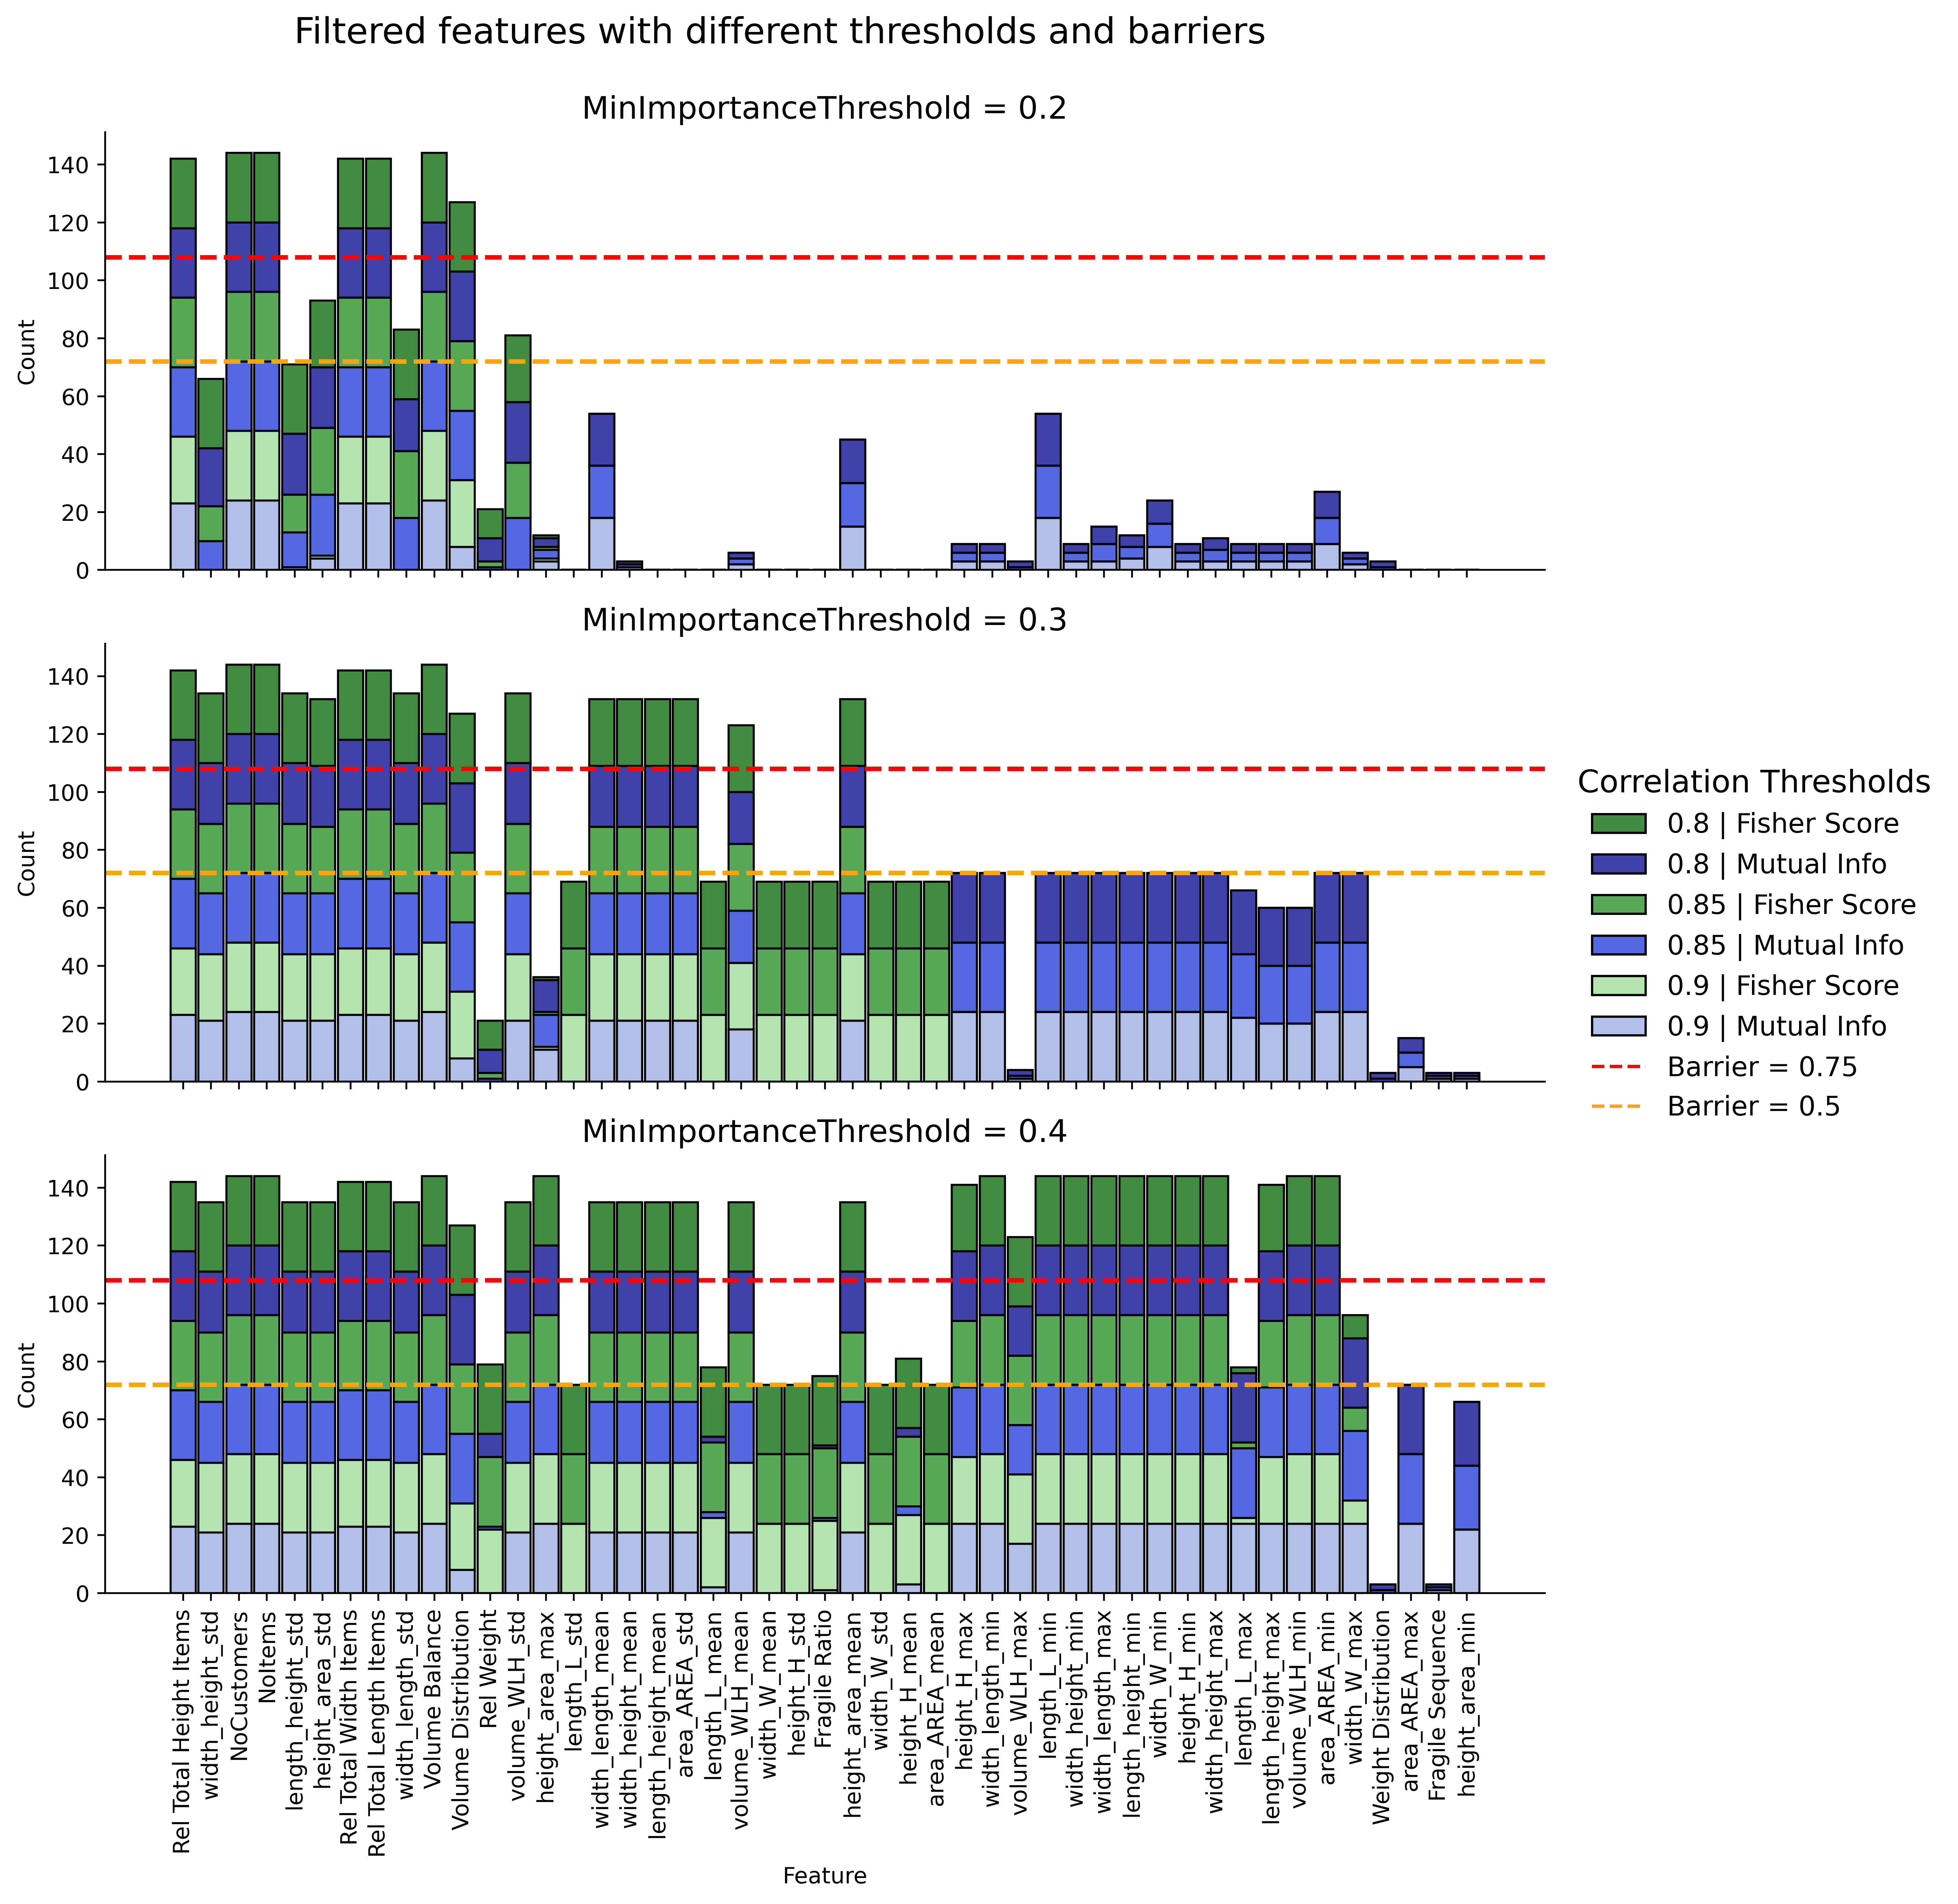
\includegraphics[width=\textwidth,height=0.75\textheight,keepaspectratio]{pictures/feature_filter_facePlot.png}
    \caption{Aggregated results from filter algorithm resulting in different drop sets.}
    \label{fig:feature_filter_parameters}
\end{figure}

\begin{table}[ht]
    \centering
    \renewcommand{\arraystretch}{0.98}
    \rotatebox{90}{
        \footnotesize
        \begin{tabular}{@{}P{0.045\paperheight}P{0.04\paperheight}P{0.07\paperheight}P{0.05\paperheight}P{0.47\paperheight}@{}}
            \toprule
            Name         & Barrier $B$ & Importance Threshold $\epsilon$ & Number Features & Features to be dropped                                                                                                                                                                                                                                                                                                                                                                                                                                                                                                                                                                                                                                        \\
            \midrule
            DropSet-50-2 & 0.50        & 0.2                             & 10              & NoCustomers, NoItems, Rel Total Height Items, Rel Total Length Items, Rel Total Width Items, Volume Balance, Volume Distribution, height-area-std, volume-WLH-std, width-length-std                                                                                                                                                                                                                                                                                                                                                                                                                                                                           \\
            \midrule
            DropSet-50-3 & 0.50        & 0.3                             & 18              & NoCustomers, NoItems, Rel Total Height Items, Rel Total Length Items, Rel Total Width Items, Volume Balance, Volume Distribution, area-AREA-std, height-area-mean, height-area-std, length-height-mean, length-height-std, volume-WLH-mean, volume-WLH-std, width-height-mean, width-height-std, width-length-mean, width-length-std                                                                                                                                                                                                                                                                                                                          \\
            \midrule
            DropSet-50-4 & 0.50        & 0.4                             & 38              & Fragile Ratio, NoCustomers, NoItems, Rel Total Height Items, Rel Total Length Items, Rel Total Width Items, Rel Weight, Volume Balance, Volume Distribution, area-AREA-min, area-AREA-std, height-H-max, height-H-mean, height-H-min, height-area-max, height-area-mean, height-area-std, length-L-max, length-L-mean, length-L-min, length-height-max, length-height-mean, length-height-min, length-height-std, volume-WLH-max, volume-WLH-mean, volume-WLH-min, volume-WLH-std, width-W-max, width-W-min, width-height-max, width-height-mean, width-height-min, width-height-std, width-length-max, width-length-mean, width-length-min, width-length-std \\
            \midrule
            DropSet-75-2 & 0.50        & 0.2                             & 7               & NoCustomers, NoItems, Rel Total Height Items, Rel Total Length Items, Rel Total Width Items, Volume Balance, Volume Distribution                                                                                                                                                                                                                                                                                                                                                                                                                                                                                                                              \\
            \midrule
            DropSet-75-3 & 0.50        & 0.3                             & 18              & NoCustomers, NoItems, Rel Total Height Items, Rel Total Length Items, Rel Total Width Items, Volume Balance, Volume Distribution, area-AREA-std, height-area-mean, height-area-std, length-height-mean, length-height-std, volume-WLH-mean, volume-WLH-std, width-height-mean, width-height-std, width-length-mean, width-length-std                                                                                                                                                                                                                                                                                                                          \\
            \midrule
            DropSet-75-4 & 0.50        & 0.4                             & 32              & NoCustomers, NoItems, Rel Total Height Items, Rel Total Length Items, Rel Total Width Items, Volume Balance, Volume Distribution, area-AREA-min, area-AREA-std, height-H-max, height-H-min, height-area-max, height-area-mean, height-area-std, length-L-min, length-height-max, length-height-mean, length-height-min, length-height-std, volume-WLH-max, volume-WLH-mean, volume-WLH-min, volume-WLH-std, width-W-min, width-height-max, width-height-mean, width-height-min, width-height-std, width-length-max, width-length-mean, width-length-min, width-length-std                                                                                     \\

            \bottomrule
        \end{tabular}}
    \caption{Feature dropsets with different parameter combinations of $\epsilon$ and $B$.}
    \label{tab:feature_dropsets}
\end{table}

\begin{table}[ht]
    \centering
    \small
    \caption{Model hyperparameters for feature selection.}
    \label{tab:hyperparams_feature_selection}
    \renewcommand{\arraystretch}{1.1}
    \begin{tabular}{@{}c P{0.3\textwidth}P{0.3\textwidth}@{}}
        \toprule
        \textbf{LR}                  & \textbf{XGB}                    & \textbf{FFNN}                      \\
        \midrule
        \kv{penalty}{l2}             & \kv{objective}{binary:logistic} & \kv{hidden\_layers}{[128, 64, 32]} \\
        \kv{C}{1.0}                  & \kv{eval\_metric}{logloss}      & \kv{dropout}{0.2}                  \\
        \kv{solver}{lbfgs}           & \kv{max\_depth}{15}             & \kv{lr}{0.001}                     \\
        \kv{max\_iter}{1000}         & \kv{n\_estimators}{500}         & \kv{batch\_size}{512}              \\
        \kv{class\_weight}{balanced} & \kv{learning\_rate}{0.05}       & \kv{epochs}{50}                    \\
        \kv{random\_state}{42}       & \kv{subsample}{0.8}             & \kv{pos\_weight}{null}             \\
        \kv{n\_jobs}{23}             & \kv{colsample\_bytree}{0.8}     & \kv{weight\_decay}{0.0}            \\
                                     & \kv{reg\_alpha}{0.0}            & \kv{batch\_size}{512}              \\
                                     & \kv{reg\_lambda}{1.0}           & \kv{device}{cpu}                   \\
                                     & \kv{enable\_categorical}{false} & \kv{random\_state}{42}             \\
                                     & \kv{tree\_method}{hist}         & \kv{n\_jobs}{23}                   \\
                                     & \kv{n\_jobs}{23}                &                                    \\
                                     & \kv{random\_state}{42}          &                                    \\
        \bottomrule
    \end{tabular}
\end{table}


\clearpage
\section{Further Feature Filter Results}
\label{app:sec:further_feature_filter}
The experiments conducted on the various drop sets, presented in Table~\ref{tab:drop_set_presentation_shortened}, included all
random and save-strategy datasets as base datasets, as well as the same set of datasets as test/prediction datasets.
In addition, all three model types were considered. This appendix section provides a more detailed discussion of the
results and highlights differences in feature filter performance.

As noted in Section~\ref{sec:feature_filter_results}, predictions from save-strategy datasets to other save-strategy datasets
(e.g., GD-Complete-WS to GD-Complete) were excluded. This is because all routes in GD-Complete are also part of GD-Complete-WS,
which would lead to misleading results by effectively evaluating the model on its training data. When focusing only on cross-predictions
between random and save-strategy datasets, the performance of drop set DS-50-4 appears even stronger, since it is not overshadowed by
the large number of random-to-random predictions.
\begin{figure}[ht]
    \centering
    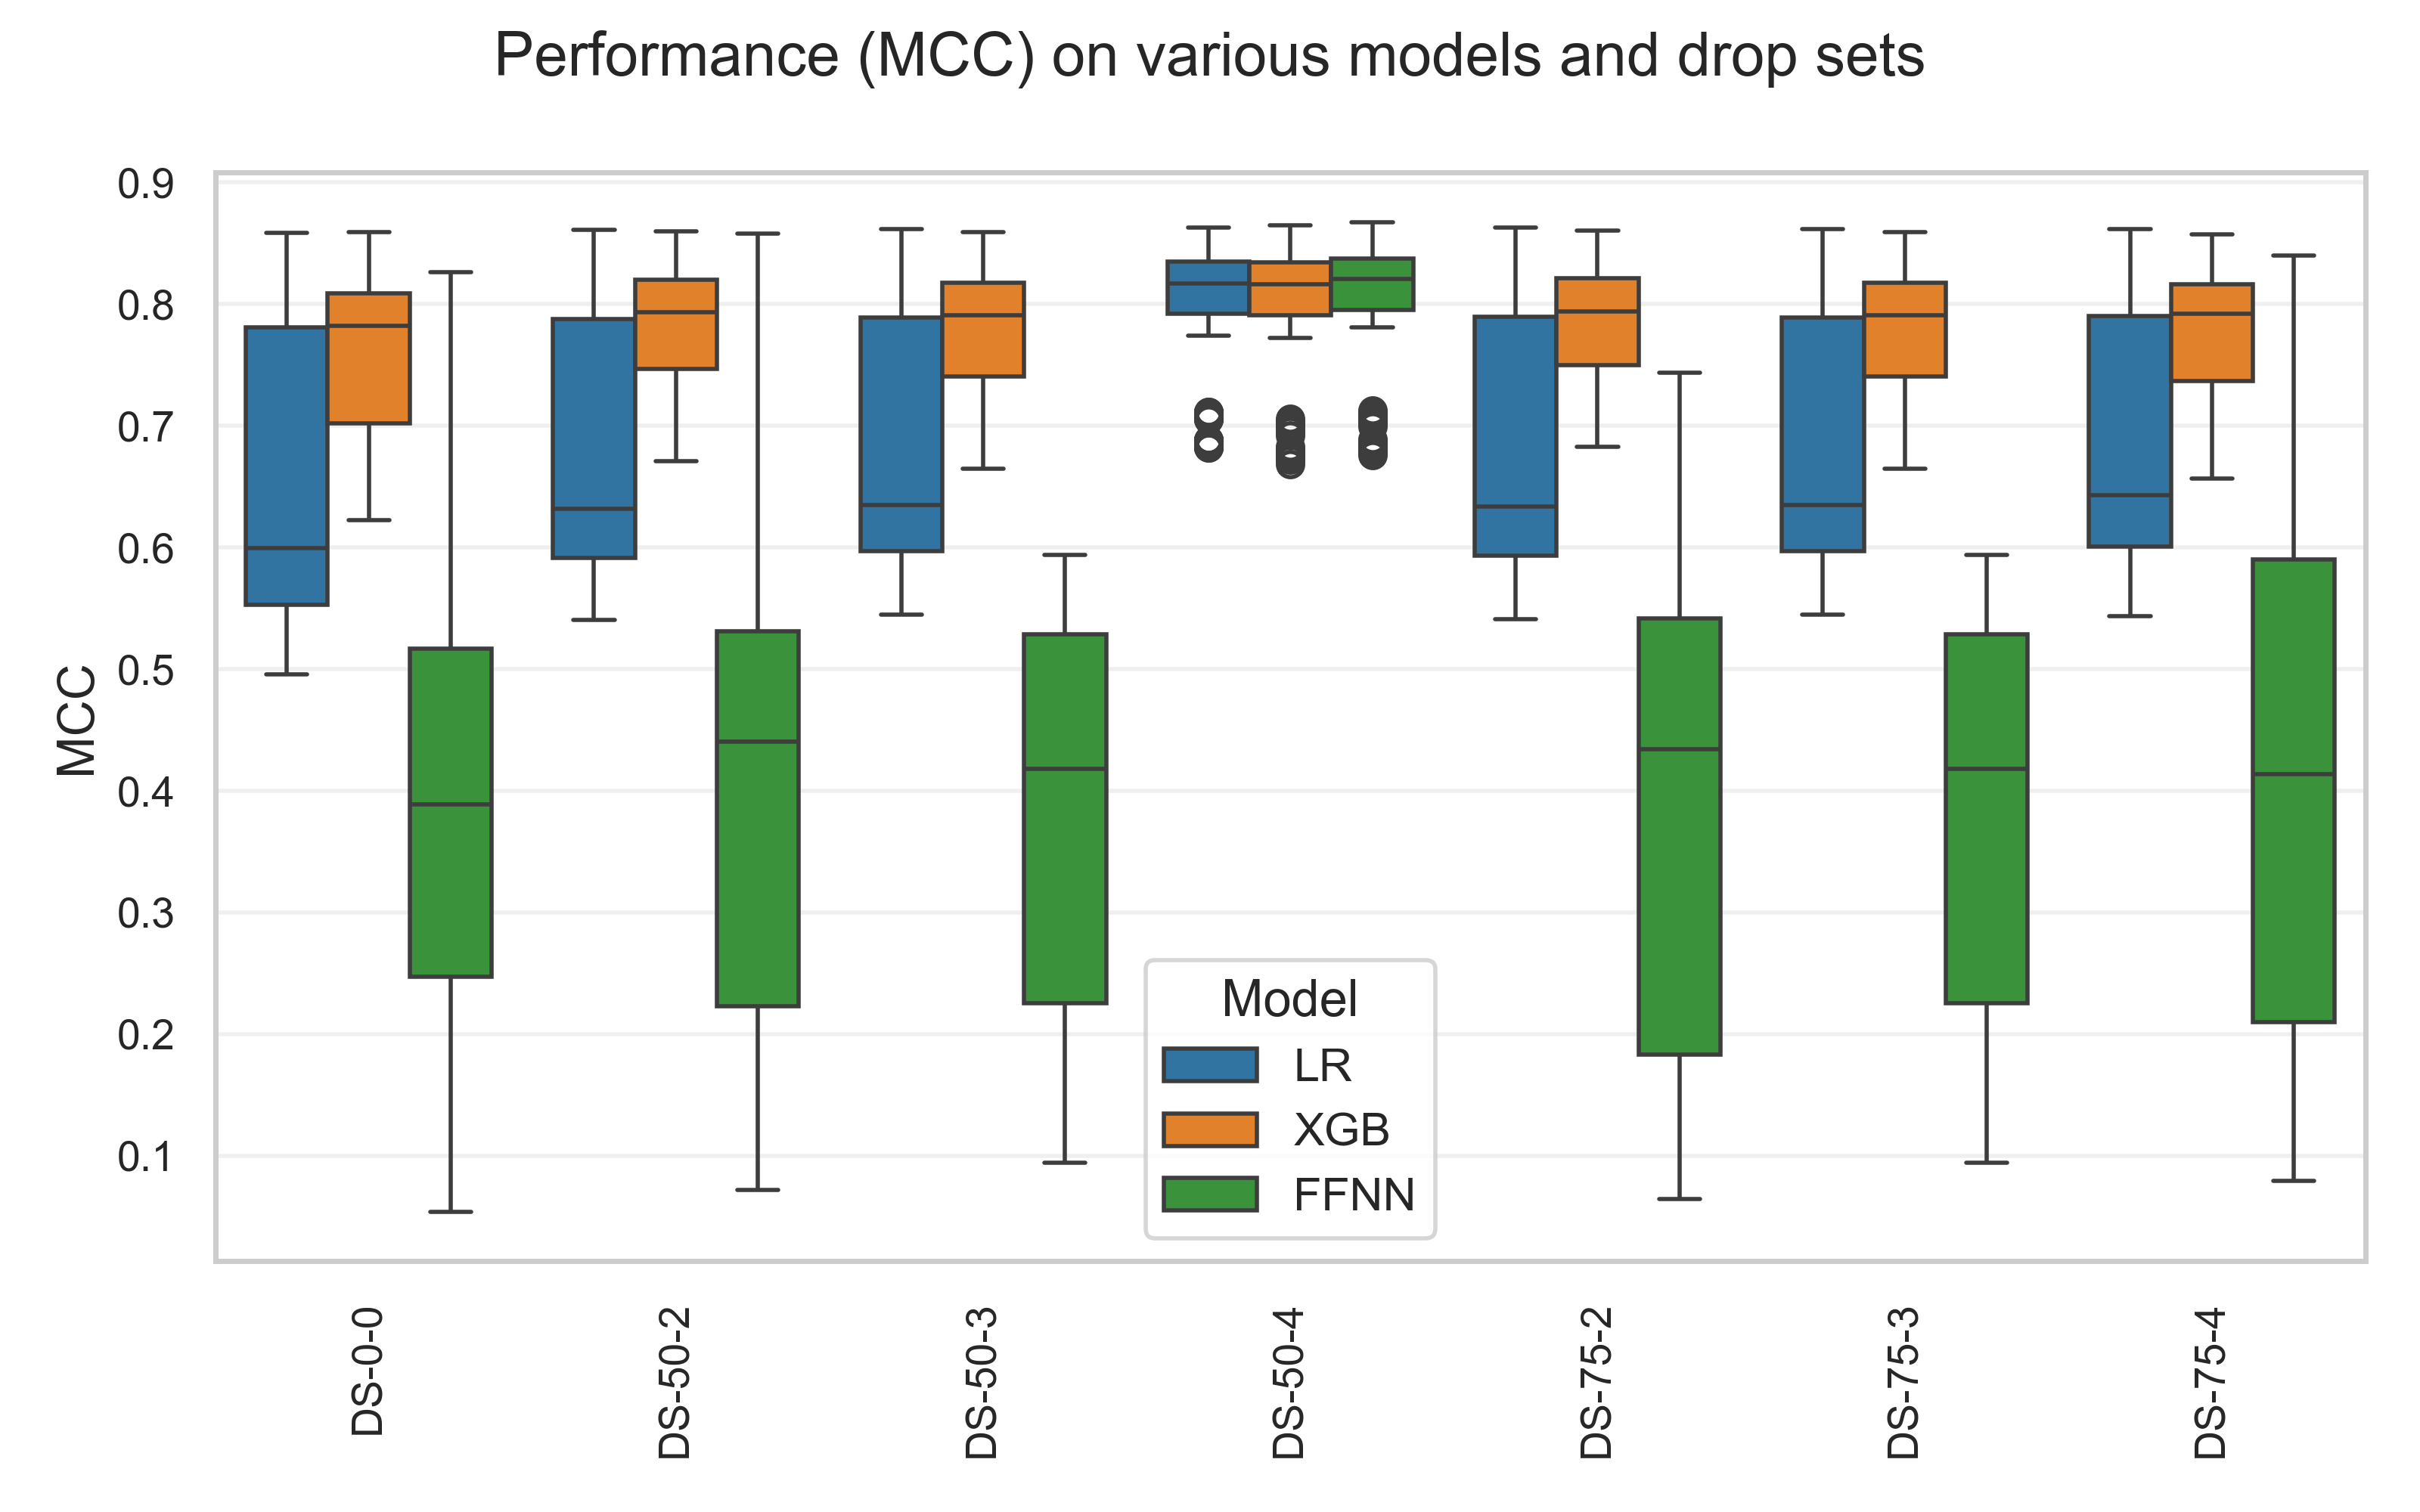
\includegraphics[width = .85\textwidth]{pictures/feature_filter/cross_performance_boxplot.png}
    \caption{Box plots of MCC performance considering only the cross performance from random to save strategy datasets and vice versa.}
    \label{fig:mcc_filter_results_cross}
\end{figure}

The mean performance metrics for the cross-predictions results are shown in the following Table~\ref{tab:featurePerformance_OnlyCrossCorrelation}.
\begin{table}[ht]
    \centering
    \begin{tabular}{lrrrrrrr}
        \toprule
        DropSet  & DS-0-0 & DS-50-2 & DS-50-3 & DS-50-4       & DS-75-2 & DS-75-3 & DS-75-4 \\
        \midrule
        MCC      & 0.60   & 0.62    & 0.61    & \textbf{0.80} & 0.61    & 0.61    & 0.62    \\
        F1-Score & 0.68   & 0.70    & 0.70    & \textbf{0.86} & 0.70    & 0.70    & 0.71    \\
        Accuracy & 0.81   & 0.81    & 0.81    & \textbf{0.92} & 0.81    & 0.81    & 0.81    \\
        AUROC    & 0.92   & 0.91    & 0.91    & \textbf{0.97} & 0.90    & 0.91    & 0.91    \\
        \bottomrule
    \end{tabular}
    \caption[Mean performance metrics on various different drop set considering only the cross-predictions from random to save strategy datasets and vice versa.]
    {Mean performance metrics on various different drop set considering only the cross-predictions from from random to save strategy datasets and vice versa.
        Bold font shows the best results for each performance score.}
    \label{tab:featurePerformance_OnlyCrossCorrelation}
\end{table}
When plotting the mean performance for each base training dataset (see Fig.~\ref{fig:mcc_filter_results_lineplot}),
the results reveal that both the XGB and LR models maintain consistently high performance across datasets. In contrast,
the FFNN model shows a significant performance drop when trained on a random dataset and applied to a save-strategy dataset.
The XGB model only performed poorly on two cases, the trimmed datasets. This can be explained by the absence of feasible
two-customer routes in these datasets, as only infeasible ones are included, making them unsuitable for further prediction tasks.
\begin{figure}[ht]
    \centering
    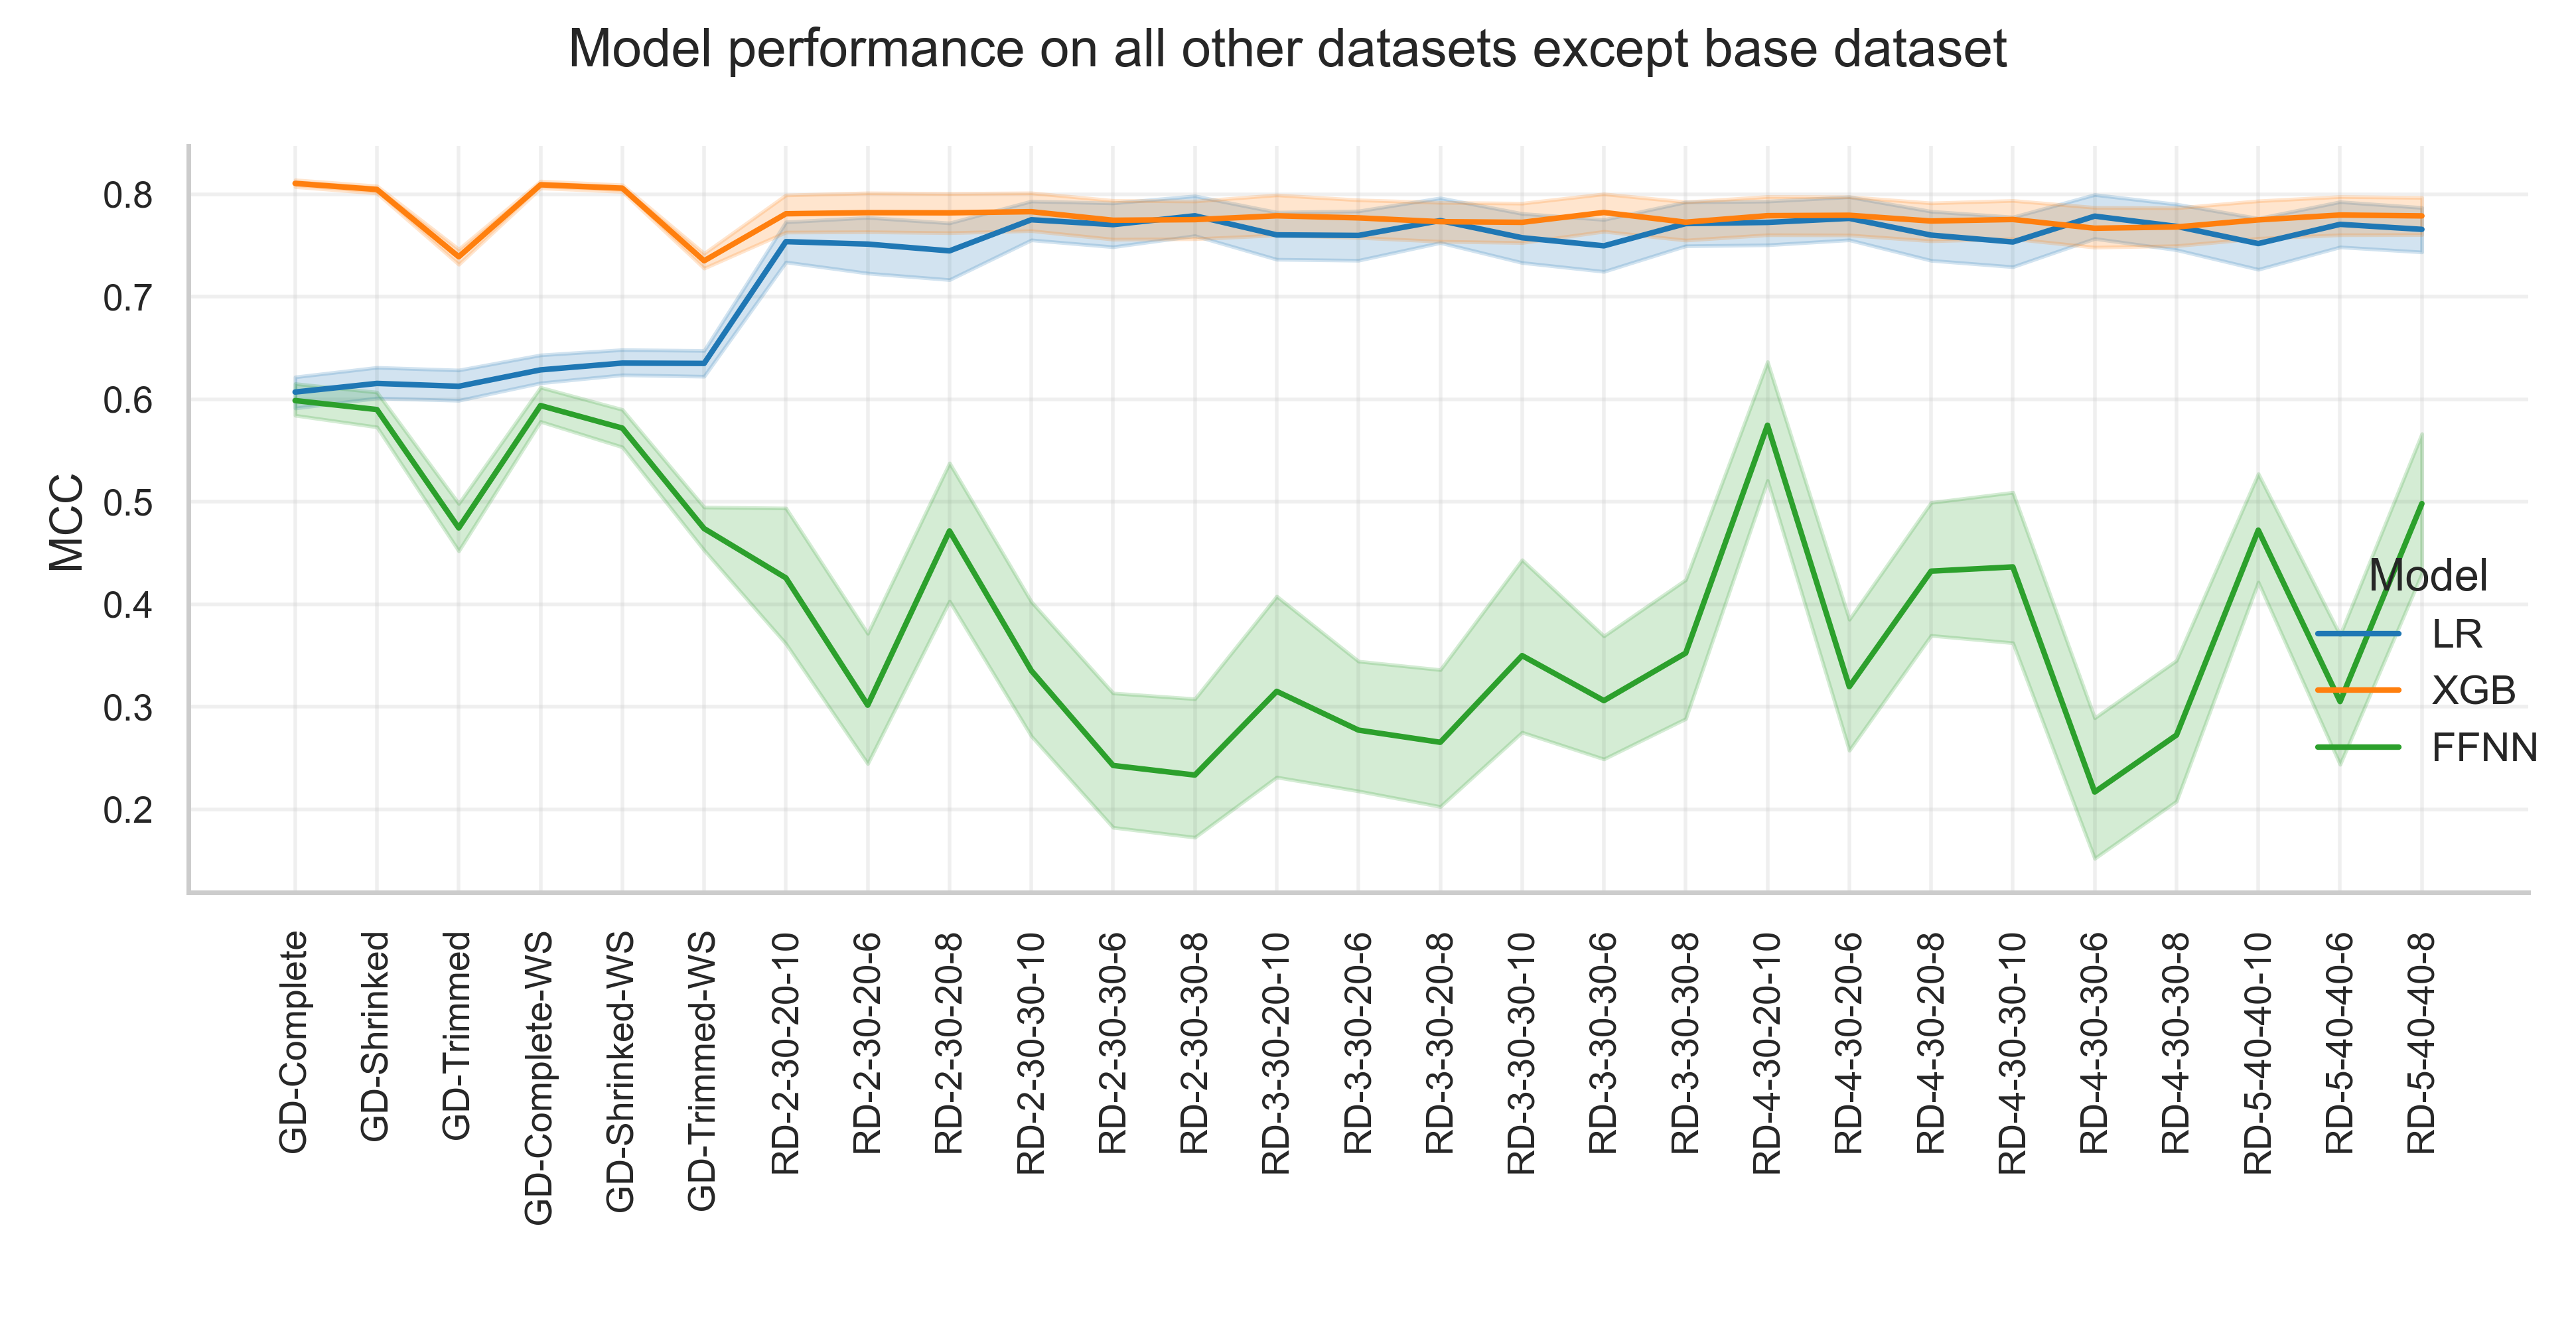
\includegraphics[width = .95\textwidth]{pictures/feature_filter/cross_performance_lineplot.png}
    \caption{Box plots of MCC performance of different feature drop sets.}
    \label{fig:mcc_filter_results_lineplot}
\end{figure}%
During the training of different models on various datasets and their subsequent predictions on the remaining datasets,
the lifetime of each model type was recorded.
For each drop set, model, and training dataset, the lifetime measurement began at model initialization and ended once
predictions were completed for all other datasets. Figure~\ref{fig:lifetime_model} highlights the substantial difference in computation time
between \gls{LR}, \gls{XGB} and \gls{FFNN} models, with the latter representing the main bottleneck in training and testing different model features.

\begin{figure}[!ht]
    \begin{center}
        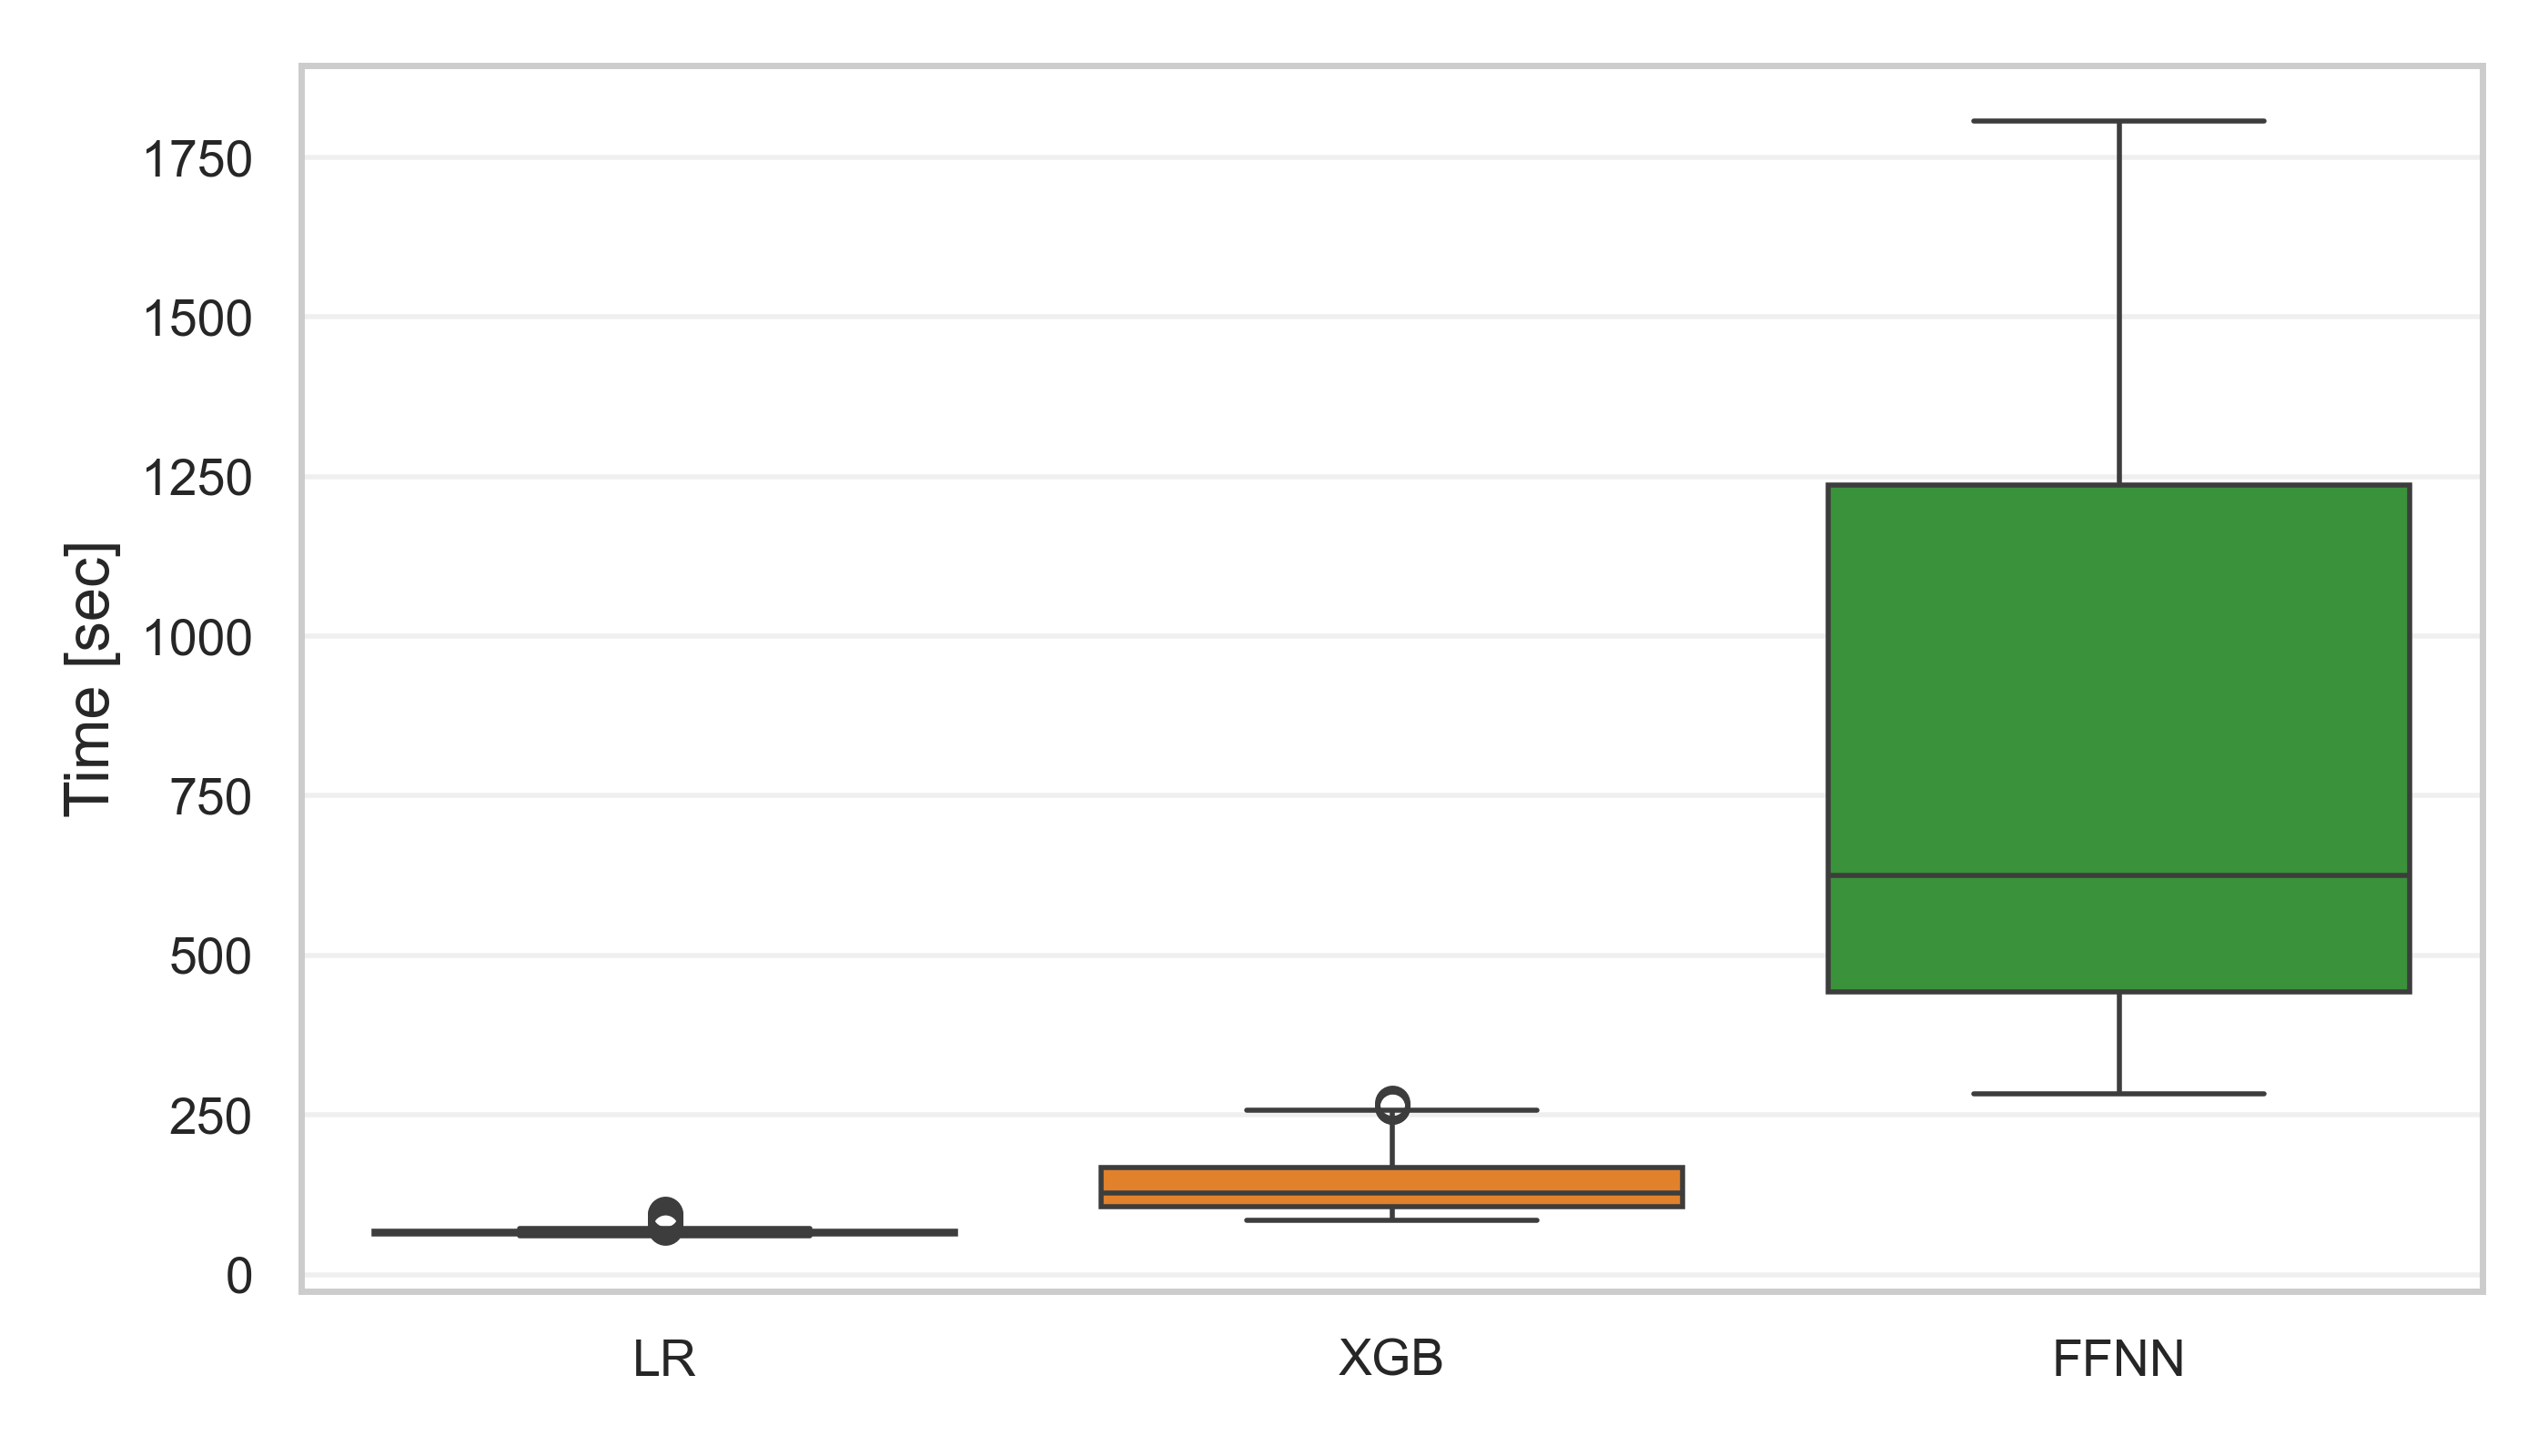
\includegraphics[width = .7\textwidth]{pictures/feature_filter/life_time_models.png}
        \caption{Life time box plots of models for training and predictions used in drop set analysis.}
        \label{fig:lifetime_model}
    \end{center}
\end{figure}

\clearpage
\section{Validation Dataset Results}
\label{app:se:validation_results}

\begin{table}[ht]
    \centering
    \small
    \begin{tabular}{llrrrr}
        \toprule
        Strategy                 & Base Dataset   & MCC            & F1-Score       & Accuracy       & AUROC          \\
        \midrule
        \multirow{6}{*}{B\&C}    & GD-Complete    & 0.731          & 0.849          & 0.865          & \textbf{0.949} \\
                                 & GD-Complete-WS & 0.736          & 0.854          & 0.868          & \textbf{0.949} \\
                                 & GD-Shrinked    & \textbf{0.737} & \textbf{0.855} & \textbf{0.869} & \textbf{0.949} \\
                                 & GD-Shrinked-WS & \textbf{0.737} & \textbf{0.857} & \textbf{0.869} & \textbf{0.949} \\
                                 & GD-Trimmed     & 0.730          & 0.854          & 0.865          & 0.947          \\
                                 & GD-Trimmed-WS  & 0.725          & 0.850          & 0.861          & 0.947          \\
        \midrule
        \multirow{21}{*}{Random} & RD-2-30-20-10  & 0.718          & 0.844          & 0.858          & 0.944          \\
                                 & RD-2-30-20-6   & 0.720          & 0.844          & 0.860          & 0.944          \\
                                 & RD-2-30-20-8   & 0.721          & 0.846          & 0.860          & 0.944          \\
                                 & RD-2-30-30-10  & 0.723          & \textbf{0.849} & 0.861          & 0.945          \\
                                 & RD-2-30-30-6   & 0.720          & 0.844          & 0.860          & 0.945          \\
                                 & RD-2-30-30-8   & 0.722          & 0.846          & 0.861          & 0.944          \\
                                 & RD-3-30-20-10  & 0.723          & \textbf{0.849} & 0.861          & 0.944          \\
                                 & RD-3-30-20-6   & 0.719          & 0.842          & 0.859          & 0.945          \\
                                 & RD-3-30-20-8   & 0.721          & 0.844          & 0.860          & 0.945          \\
                                 & RD-3-30-30-10  & 0.722          & 0.848          & 0.861          & 0.945          \\
                                 & RD-3-30-30-6   & 0.722          & 0.846          & 0.861          & 0.945          \\
                                 & RD-3-30-30-8   & 0.722          & 0.846          & 0.861          & 0.945          \\
                                 & RD-4-30-20-10  & 0.720          & 0.845          & 0.859          & 0.944          \\
                                 & RD-4-30-20-6   & 0.718          & 0.842          & 0.859          & 0.945          \\
                                 & RD-4-30-20-8   & 0.719          & 0.845          & 0.859          & 0.944          \\
                                 & RD-4-30-30-10  & 0.722          & 0.848          & 0.861          & 0.945          \\
                                 & RD-4-30-30-6   & \textbf{0.725} & 0.848          & \textbf{0.863} & \textbf{0.946} \\
                                 & RD-4-30-30-8   & \textbf{0.725} & 0.848          & \textbf{0.862} & \textbf{0.946} \\
                                 & RD-5-40-40-10  & 0.723          & 0.848          & 0.861          & 0.945          \\
                                 & RD-5-40-40-6   & \textbf{0.725} & 0.848          & \textbf{0.862} & \textbf{0.946} \\
                                 & RD-5-40-40-8   & 0.724          & 0.848          & \textbf{0.862} & \textbf{0.946} \\
        \bottomrule
    \end{tabular}
    \caption[Average performance metrics on the validation data set.]{Average performance metrics on the validation data set.
        For each strategy group the metrics with the highest values are marked bold, if several columns have the same highest value
        all of them marked.}
    \label{tab:featurePerformance_validationDataset}
\end{table}

\clearpage
\section{Parking Lot}
\begin{table}[ht]
    \centering
    \begin{tabular}{c c c c c c c}
        \toprule
        Model                          & Strategy & Name       & \gls{MCC}-Score & \gls{AUROC} & F1-Score & Accuracy \\
        \midrule
        \multirow{2}{*}{\gls{LR}}      & Random   & RD-4-20-30 & 0.6             & 0.87        & 0.9      & 0.8      \\
                                       & Save     & Complete   & 0.6             & 0.87        & 0.9      & 0.8      \\
        \midrule
        \multirow{2}{*}{Decision Tree} & Random   & RD-4-20-30 & 0.6             & 0.87        & 0.9      & 0.8      \\
                                       & Save     & Complete   & 0.6             & 0.87        & 0.9      & 0.8      \\
        \midrule
        \multirow{2}{*}{\gls{FFNN}}    & Random   & RD-4-20-30 & 0.6             & 0.87        & 0.9      & 0.8      \\
                                       & Save     & Complete   & 0.6             & 0.87        & 0.9      & 0.8      \\

        \bottomrule
    \end{tabular}
    \caption{Presentatione of final datasets and feature selection}
    \label{tab:final_dataset_features}
\end{table}
\clearpage


\section{Parameterstudy}

\subsection{NoClasifier Variant}
\label{app:subsec:parameterstudy_noclassifier}

\begin{figure}[!ht]
    \centering
    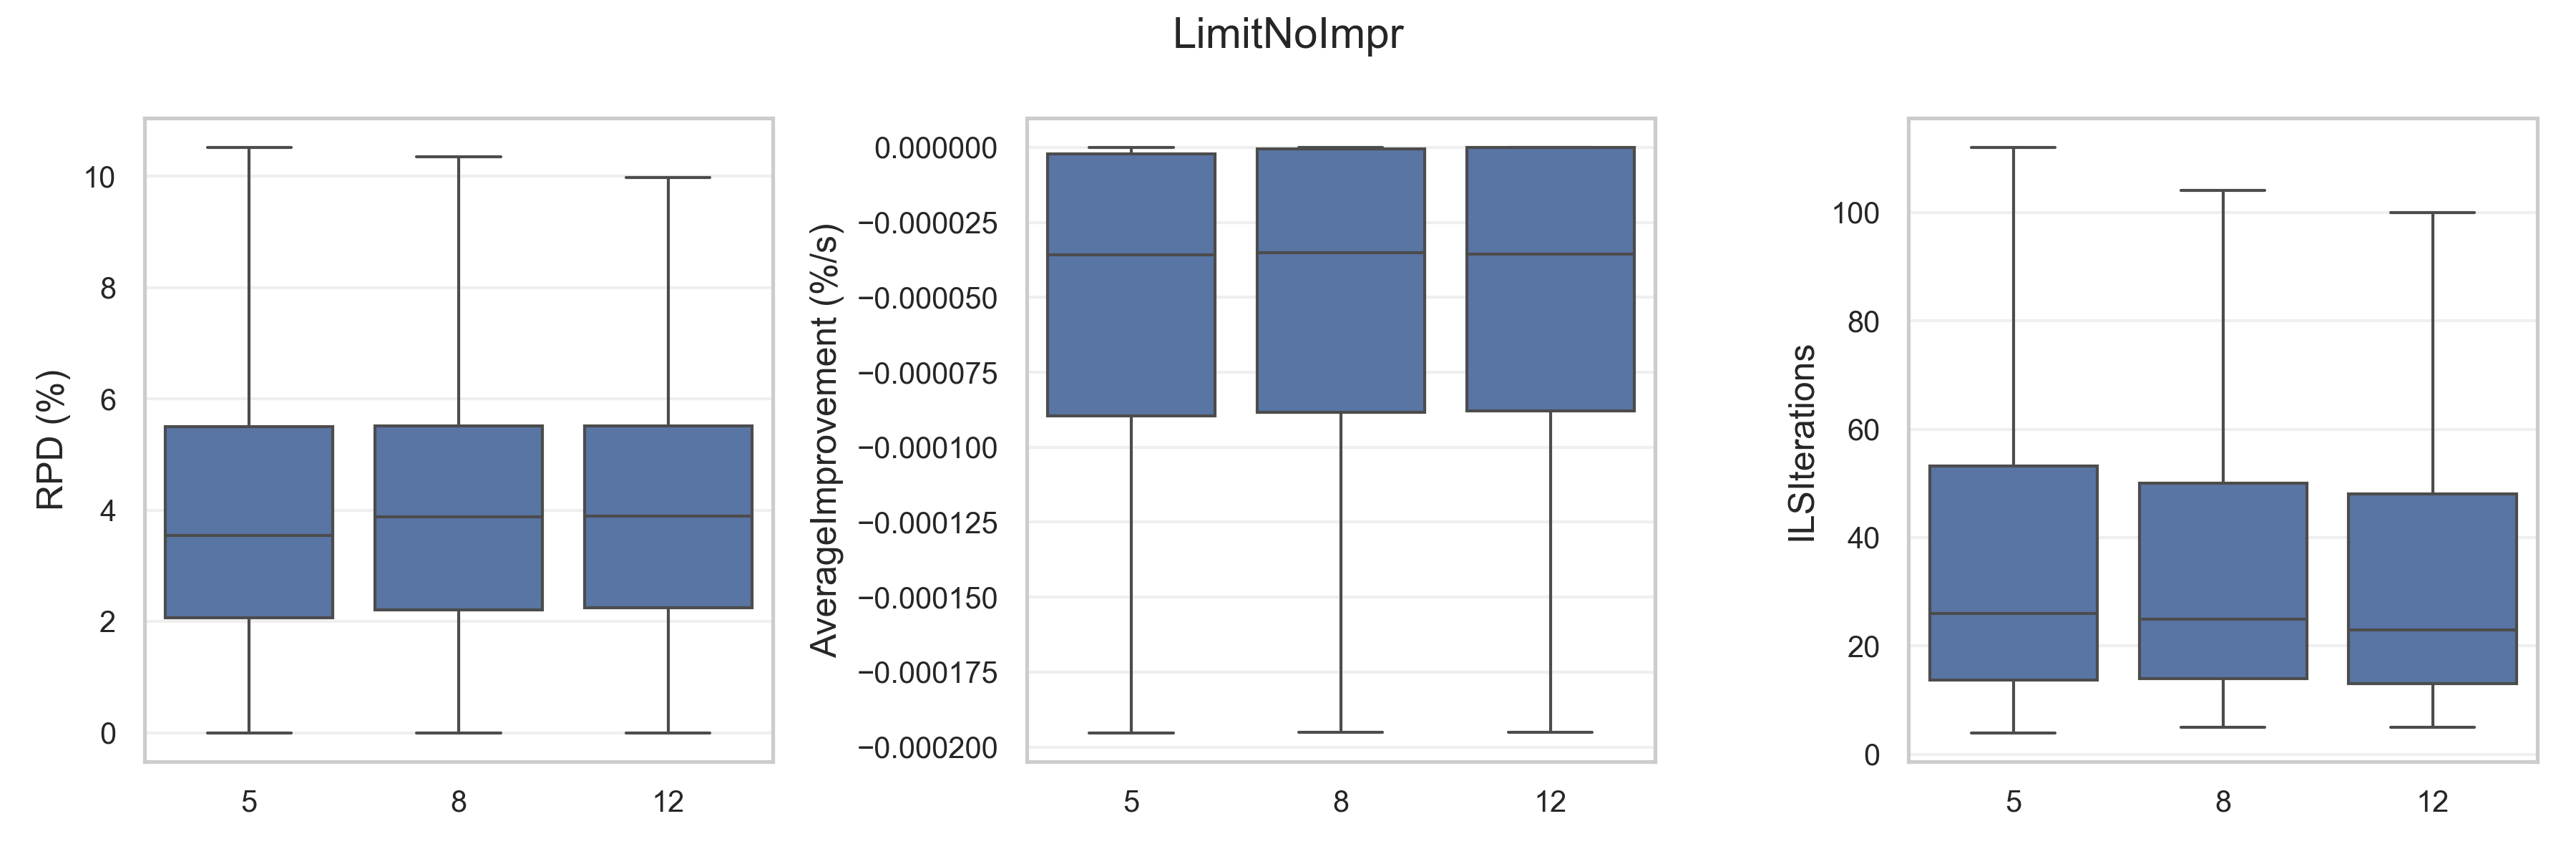
\includegraphics[width=\textwidth]{pictures/parameter_study/LimitNoImpr_base_parameter_study.png}
    \caption{Parameterstudy of LimitNoImpr divided in two groups based on the average iterations.}
    \label{fig:parameterstudy_NoClassifier_limitNoImpr}
\end{figure}

\begin{figure}[!ht]
    \centering
    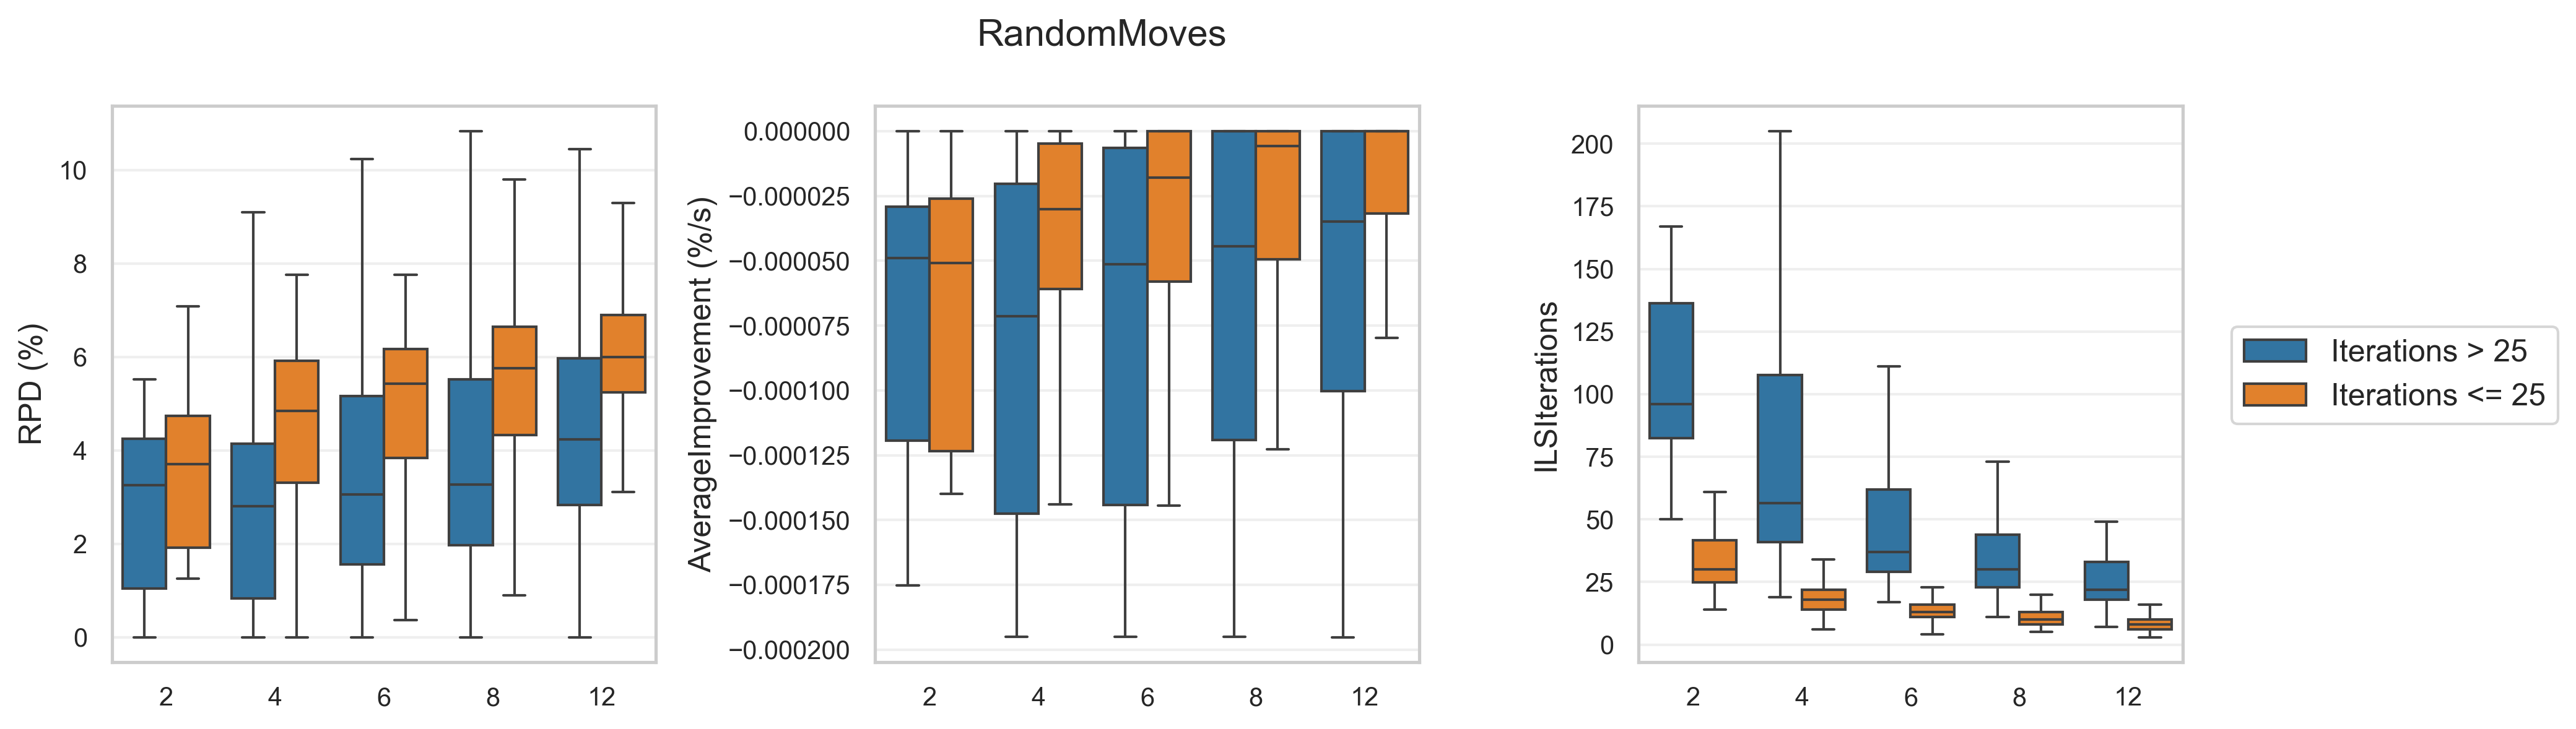
\includegraphics[width=\textwidth]{pictures/parameter_study/RandomMoves_base_parameter_study.png}
    \caption{Parameterstudy of RandomMoves divided in two groups based on the average iterations.}
    \label{fig:parameterstudy_NoClassifier_RandomMoves}
\end{figure}

\begin{figure}[!ht]
    \centering
    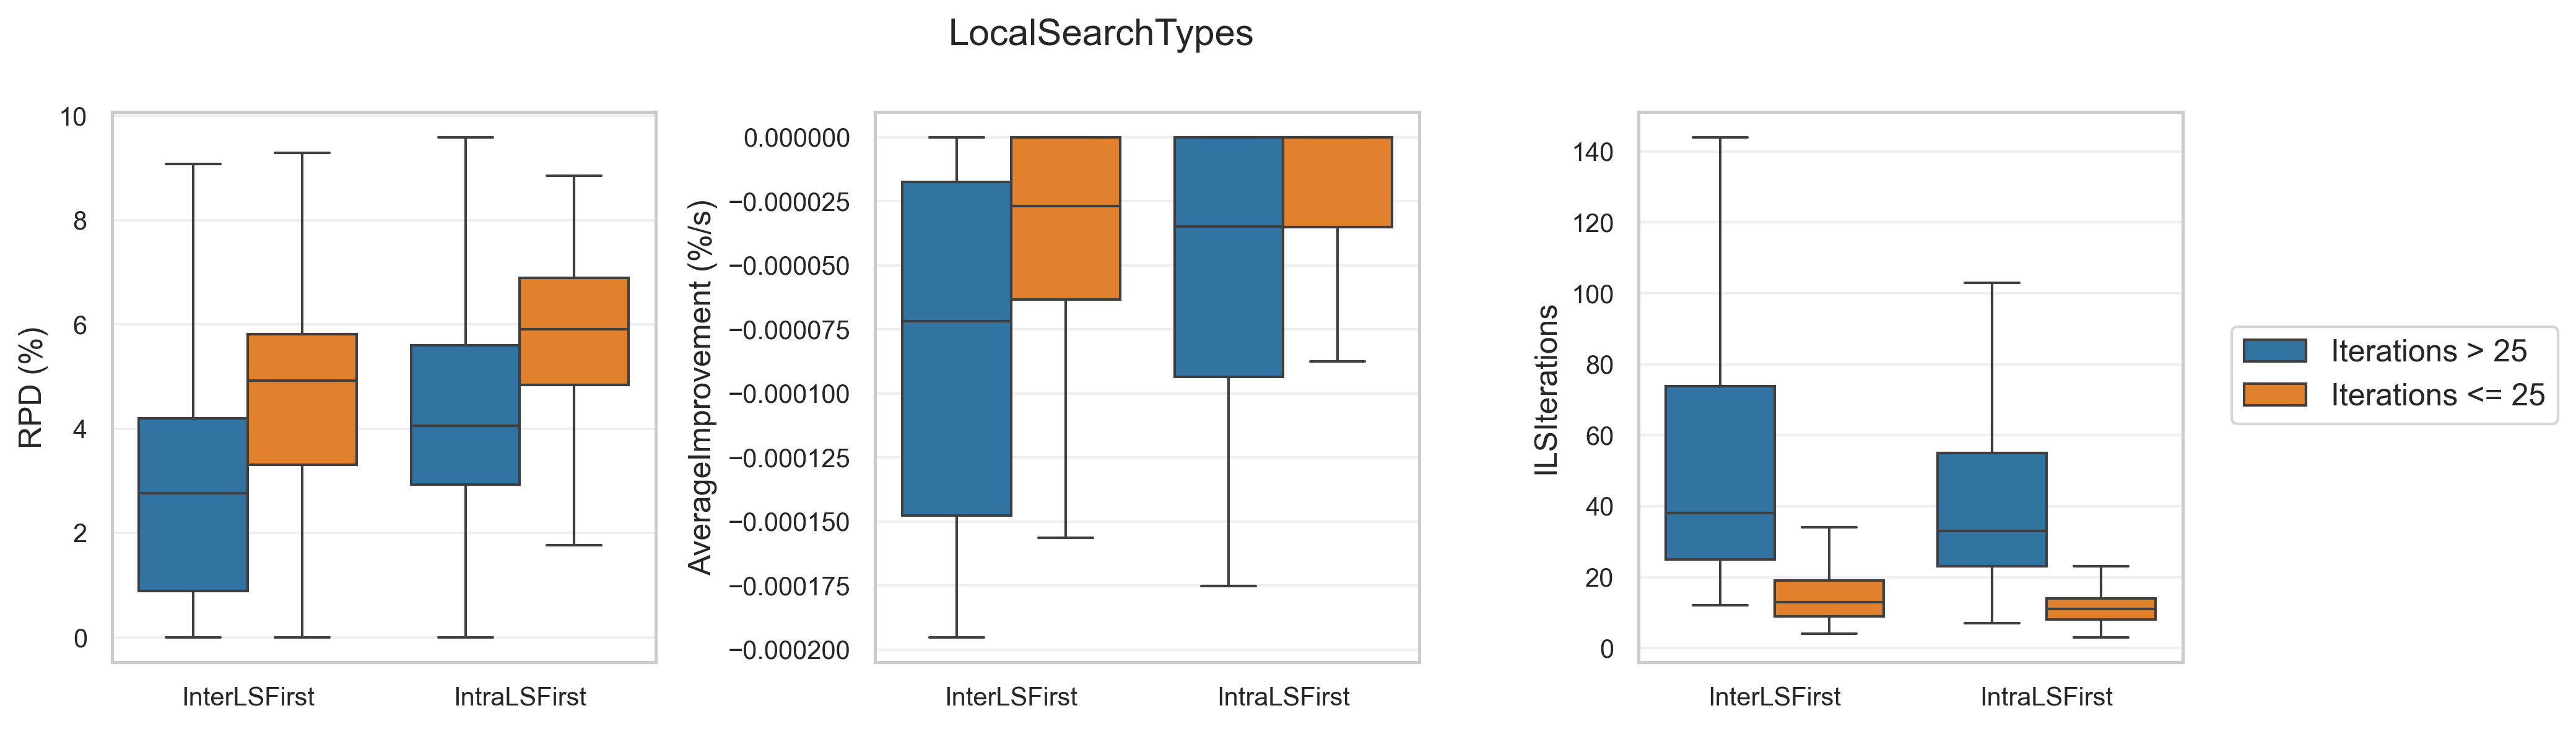
\includegraphics[width=\textwidth]{pictures/parameter_study/LocalSearchTypes_base_parameter_study.png}
    \caption{Parameterstudy of the order of local search neighborhoods divided in two groups based on the average iterations.}
    \label{fig:parameterstudy_NoClassifier_localSearch}
\end{figure}

\begin{figure}[!ht]
    \centering
    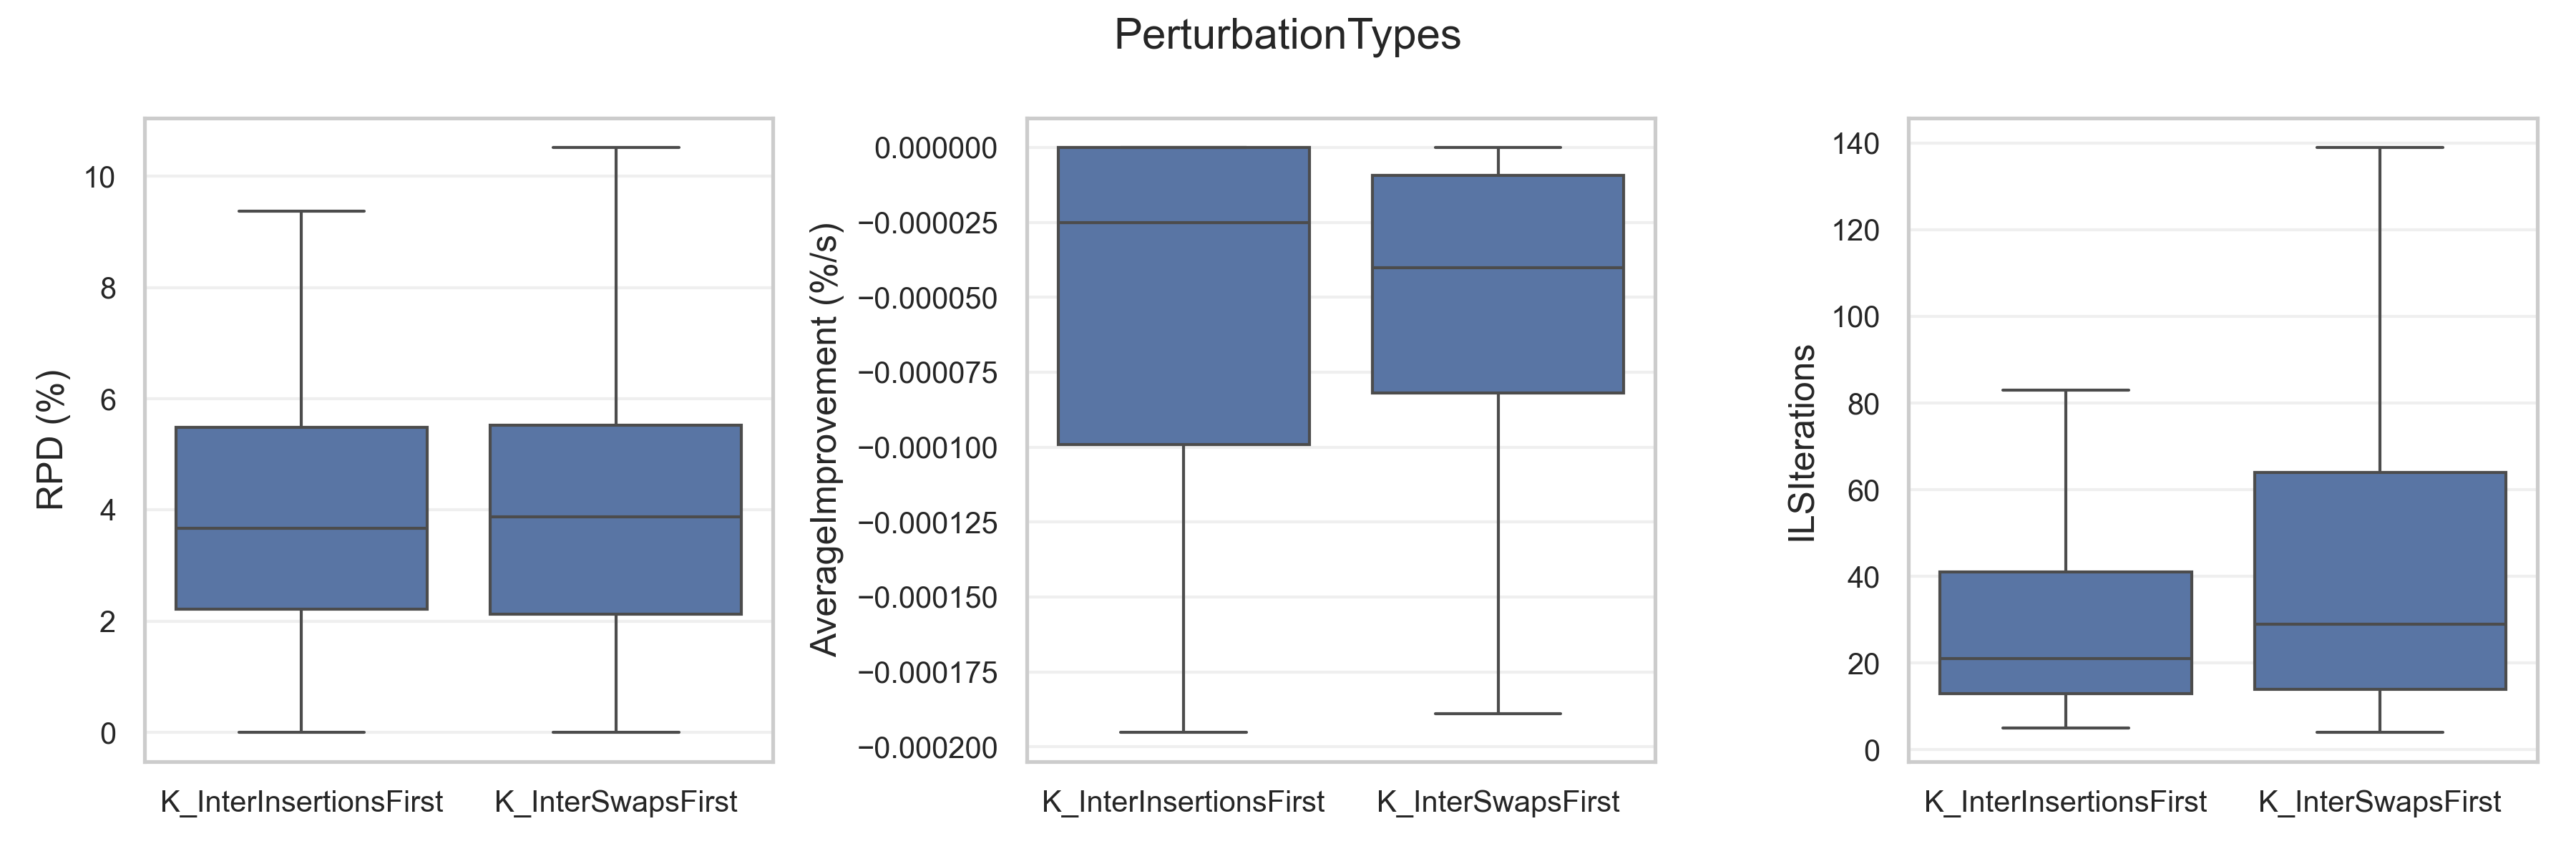
\includegraphics[width=\textwidth]{pictures/parameter_study/PerturbationTypes_base_parameter_study.png}
    \caption{Parameterstudy of the set and order of perturbation neighborhoods divided in two groups based on the average iterations.}
    \label{fig:parameterstudy_NoClassifier_perturbation}
\end{figure}

\subsection{SpeedUp Variant}
\label{app:subsec:parameterstudy_SpeedUp}

\clearpage
\section{Branch-and-Cut Results}

The following two tables summarize the results of the branch-and-cut algorithm used for the the retrieval of train datasets
from save strategy. The following table explains each column header:

\begin{table}[ht]
    \centering
    \begin{tabular}{C{0.2\textwidth}C{0.74\textwidth}}
        \toprule
        Column Header & Description                                                    \\
        \midrule
        $C^*$         & Best objective (Costs)                                         \\
        Gap           & Gap to \gls{LB} in B\&C procedure                              \\
        $K^*$         & Final number of routes                                         \\
        $N$           & Number of explored branch-and-bound nodes                      \\
        $t$           & Runtime of algorithm; TL = Timelimit (28880 sec)               \\
        $C_0$         & Objective of start solution                                    \\
        $K_0$         & Number of routes start solution                                \\
        $\Delta BKS$  & Percentage difference of objective to best known solution (\%) \\
        \bottomrule
    \end{tabular}
    \caption{Column header description for B\&C results.}
    \label{tab:column_header_description_bc}
\end{table}

The results for \gendreauDataSetText are shown in Table~\ref{tab:bc_results_gendreau} and for \krebsADataSetText in Table~\ref{tab:bc_results_krebs}.
Both instances are sorted in the groups lightweigt (L) and heavyweight (H) labeled by the instance names, indicating if the average weight
requested by a customer is above (H) or under (L) the average of all instances, indicating the complexity to solve the instances optimally.
As weight is a one dimensional loading constraint factor, the feasbility check is fast. The results can be divided by this weight label
pretty perfectly in instances being solved optimally (H), or which needed a long run time and/ or and not solved optimally (L).
The solutions for \krebsADataSetText are categorized in three groups A, B and C classifying the solution process. Each label is shown
by the best objective $C^*$. The labels have the following meaning:
\begin{itemize}
    \item A : The solution process ran without complications.
    \item B : The final solution could not be created, concrete number of vehicles $K^*$ is unknown, but Gap and $C^*$ could be retrieved from Gurobi logging file.
    \item C : Only the start solution was created, leading to missing values for the main branch-and-cut algorithm. No concrete runtime $t$ could be determined.
\end{itemize}

Applying the exact algorithm from \cite{tamke_branch-and-cut_2024} to the \krebsADataSetText dataset is novel for this dataset.
The average gap across this subset of instances is 3.14\%, resulting in many optimal solutions being found.\footcite[cf.][]{tamke_branch-and-cut_2024}
The objectives cant be compared to initially published results of \cite{krebs_advanced_2021}, as the \gls{3L-CVRP} was solved rather than the initial \gls{3L-VRPTW}.\footcite[cf.][pp. 858–864]{krebs_advanced_2021}

\begin{table}[!h]
    \centering
    \small
    \begin{tabular}{lrrrrll}
        \toprule
        Instance Name       & $C^*$   & Gap  & $K^*$ & $N$     & $t$   & $\Delta BKS$    \\
        \midrule
        $\text{E016-03m}^H$ & 301.66  & 0.00 & 4     & 4290    & 21    & $\text{0.0}^e$  \\
        $\text{E016-05m}^H$ & 334.96  & 0.00 & 5     & 53      & 1     & $\text{0.0}^a$  \\
        $\text{E021-04m}^H$ & 385.53  & 0.00 & 4     & 84225   & 532   & $\text{0.0}^d$  \\
        $\text{E021-06m}^H$ & 430.88  & 0.00 & 6     & 98      & 5     & $\text{0.0}^e$  \\
        $\text{E022-04g}^H$ & 427.56  & 0.00 & 5     & 138703  & 1024  & $\text{0.0}^e$  \\
        $\text{E022-06m}^H$ & 498.16  & 0.00 & 6     & 726     & 11    & $\text{0.0}^c$  \\
        $\text{E023-03g}^L$ & 757.88  & 0.00 & 5     & 1434923 & 4226  & $\text{0.0}^e$  \\
        $\text{E023-05s}^L$ & 798.65  & 0.01 & 6     & 2614340 & TL    & $\text{0.0}^e$  \\
        $\text{E026-08m}^H$ & 630.13  & 0.00 & 8     & 4604    & 61    & $\text{0.0}^b$  \\
        $\text{E030-03g}^L$ & 783.79  & 0.17 & 6     & 1153008 & TL    & $\text{1.88}^e$ \\
        $\text{E030-04s}^L$ & 728.32  & 0.16 & 7     & 1176116 & TL    & $\text{0.0}^e$  \\
        $\text{E031-09h}^H$ & 610.23  & 0.00 & 9     & 394216  & 10598 & $\text{0.0}^b$  \\
        $\text{E033-03n}^L$ & 2649.00 & 0.14 & 6     & 564692  & TL    & $\text{1.22}^e$ \\
        $\text{E033-04g}^L$ & 1337.17 & 0.25 & 7     & 432649  & TL    & $\text{1.24}^e$ \\
        $\text{E033-05s}^L$ & 1327.09 & 0.25 & 7     & 298863  & TL    & $\text{6.13}^e$ \\
        $\text{E036-11h}^H$ & 698.61  & 0.00 & 11    & 20025   & 325   & $\text{0.0}^a$  \\
        $\text{E041-14h}^H$ & 871.63  & 0.03 & 14    & 420758  & TL    & $\text{0.6}^c$  \\
        $\text{E045-04f}^L$ & 1204.07 & 0.18 & 10    & 306014  & TL    & $\text{0.18}^d$ \\
        $\text{E051-05e}^L$ & 726.20  & 0.19 & 10    & 305879  & TL    & $\text{1.27}^e$ \\
        $\text{E072-04f}^L$ & 567.64  & 0.24 & 15    & 162320  & TL    & $\text{0.0}^d$  \\
        $\text{E076-07s}^L$ & 1040.77 & 0.25 & 15    & 197632  & TL    & $\text{0.0}^d$  \\
        $\text{E076-08s}^L$ & 1134.70 & 0.26 & 16    & 222779  & TL    & $\text{0.14}^d$ \\
        $\text{E076-10e}^L$ & 1170.51 & 0.31 & 17    & 199955  & TL    & $\text{7.96}^d$ \\
        $\text{E076-14s}^H$ & 1121.85 & 0.13 & 16    & 168907  & TL    & $\text{2.69}^d$ \\
        $\text{E101-08e}^L$ & 1375.07 & 0.29 & 20    & 162886  & TL    & $\text{2.74}^d$ \\
        $\text{E101-10c}^L$ & 1544.02 & 0.28 & 22    & 229882  & TL    & $\text{0.91}^d$ \\
        $\text{E101-14s}^L$ & 1576.76 & 0.33 & 23    & 135945  & TL    & $\text{7.11}^d$ \\
        \bottomrule
    \end{tabular}
    \caption{B\&C Results for obtaining save strategy dataset from \gendreauDataSet.}
    \label{tab:bc_results_gendreau}
\end{table}

The publisher for best known solution(BKS) for the \gendreauDataSetText is indicated by the small letter
next to the instance name. In this comparison all published papers were considered, which use the same loading constraint set $\mathcal{G}$.

\newcommand{\datasetPos}[2]{%
{#1} : {#2}
}
\begin{table}[ht]
    \centering
    \renewcommand{\arraystretch}{1.05}
    \begin{tabular}{@{}lll@{}}
        \multicolumn{2}{c}{\datasetPos{a}{\cite{tarantilis_hybrid_2009}}} & \datasetPos{b}{\cite{wang_two_2010}}                                                              \\
        \datasetPos{c}{\cite{bortfeldt_hybrid_2012}}                      & \datasetPos{d}{\cite{zhang_evolutionary_2015}} & \datasetPos{e}{\cite{tamke_branch-and-cut_2024}} \\
    \end{tabular}
\end{table}

\begin{table}[ht]
    \small
    \centering
    \begin{tabular}{llrrrlrr}
        \toprule
        Instance Name                  & $C^*$              & Gap  & $K^*$ & $N$    & $t$   & $C_0$   & $K_0$ \\
        \midrule
        $\text{012-n020-m200-bt100}^L$ & $\text{311.78}^A$  & 0.00 & 2     & 1      & 10753 & 467.39  & 5     \\
        $\text{038-n020-m200-bt10}^L$  & $\text{347.45}^A$  & 0.00 & 2     & 1      & 8019  & 543.34  & 6     \\
        $\text{039-n020-m200-bt10}^L$  & $\text{337.87}^A$  & 0.00 & 2     & 1      & 11757 & 488.54  & 5     \\
        $\text{052-n020-m200-bt10}^L$  & $\text{289.63}^A$  & 0.00 & 2     & 1      & 14972 & 502.17  & 6     \\
        $\text{054-n020-m200-bt10}^L$  & $\text{324.87}^A$  & 0.00 & 2     & 1      & 7881  & 551.42  & 5     \\
        $\text{059-n020-m200-bt100}^L$ & $\text{335.94}^A$  & 0.00 & 2     & 1      & 7884  & 514.88  & 6     \\
        $\text{069-n060-m200-bt10}^H$  & $\text{1152.87}^B$ & 0.22 & 15    & 84340  & TL    & 1169.69 & 15    \\
        $\text{076-n060-m200-bt3}^L$   & $\text{nan}^C$     & NaN  & NaN   & NaN    & -1    & 682.00  & 5     \\
        $\text{081-n060-m200-bt10}^L$  & $\text{565.54}^A$  & 0.00 & 3     & 3114   & 10180 & 666.61  & 4     \\
        $\text{086-n060-m200-bt100}^L$ & $\text{578.71}^A$  & 0.00 & 4     & 537    & 8518  & 651.16  & 5     \\
        $\text{116-n060-m200-bt100}^L$ & $\text{568.14}^A$  & 0.00 & 4     & 14     & 11053 & 630.05  & 5     \\
        $\text{117-n060-m200-bt100}^L$ & $\text{623.74}^A$  & 0.00 & 4     & 17208  & 26618 & 656.68  & 5     \\
        $\text{126-n060-m200-bt10}^H$  & $\text{1226.45}^A$ & 0.23 & 15    & 213408 & TL    & 1241.24 & 15    \\
        $\text{137-n060-m200-bt3}^L$   & $\text{538.62}^A$  & 0.00 & 3     & 6      & 11338 & 635.56  & 4     \\
        $\text{141-n060-m200-bt10}^L$  & $\text{619.35}^A$  & 0.00 & 4     & 4926   & 13948 & 693.73  & 5     \\
        $\text{149-n060-m200-bt100}^L$ & $\text{521.33}^B$  & 0.00 & NaN   & 321    & 22028 & 611.68  & 4     \\
        $\text{156-n060-m200-bt10}^H$  & $\text{1097.58}^B$ & 0.25 & 14    & 67164  & TL    & 1070.95 & 14    \\
        $\text{161-n060-m200-bt100}^H$ & $\text{1106.37}^B$ & 0.21 & 14    & 125245 & TL    & 1082.66 & 13    \\
        $\text{172-n060-m200-bt10}^L$  & $\text{563.26}^B$  & 0.00 & NaN   & 8661   & 22715 & 608.35  & 5     \\
        $\text{204-n100-m200-bt10}^L$  & $\text{733.05}^A$  & 0.00 & 4     & 25340  & 24701 & 787.06  & 5     \\
        $\text{215-n100-m200-bt3}^H$   & $\text{1238.86}^B$ & 0.10 & 14    & 87846  & TL    & 1287.75 & 13    \\
        $\text{227-n100-m200-bt3}^L$   & $\text{689.9}^A$   & 0.00 & 4     & 3079   & 2591  & 730.08  & 4     \\
        $\text{228-n100-m200-bt3}^L$   & $\text{704.05}^A$  & 0.00 & 5     & 24075  & 10046 & 750.65  & 5     \\
        $\text{245-n100-m200-bt3}^L$   & $\text{937.28}^B$  & 0.03 & NaN   & 83475  & TL    & 963.05  & 9     \\
        $\text{272-n100-m200-bt3}^L$   & $\text{959.23}^B$  & 0.05 & NaN   & 8420   & TL    & 1106.01 & 11    \\
        $\text{276-n100-m200-bt10}^H$  & $\text{1230.19}^A$ & 0.14 & 15    & 126965 & TL    & 1231.91 & 15    \\
        $\text{294-n100-m200-bt10}^L$  & $\text{678.06}^A$  & 0.00 & 3     & 15     & 22781 & 769.09  & 5     \\
        $\text{297-n100-m200-bt100}^L$ & $\text{746.4}^A$   & 0.00 & 4     & 22161  & 28286 & 783.66  & 5     \\
        $\text{299-n100-m200-bt100}^L$ & $\text{784.5}^B$   & 0.00 & NaN   & 31547  & 20498 & 831.21  & 5     \\
        $\text{386-n060-m400-bt100}^L$ & $\text{540.28}^A$  & 0.00 & 3     & 140    & 19854 & 936.23  & 10    \\
        $\text{390-n060-m400-bt100}^L$ & $\text{607.91}^B$  & 0.00 & NaN   & 1      & 12800 & 967.73  & 10    \\
        $\text{415-n060-m400-bt10}^L$  & $\text{577.24}^B$  & 0.00 & NaN   & 657    & 16734 & 873.01  & 9     \\
        $\text{423-n060-m400-bt3}^H$   & $\text{1014.38}^B$ & 0.00 & NaN   & 1      & 10191 & 1534.87 & 23    \\
        $\text{438-n060-m400-bt3}^L$   & $\text{639.95}^B$  & 0.00 & 5     & 5575   & 16971 & 809.97  & 7     \\
        $\text{499-n100-m400-bt3}^L$   & $\text{767.32}^B$  & 0.00 & 4     & 17961  & TL    & 945.93  & 7     \\
        $\text{527-n100-m400-bt3}^L$   & $\text{737.34}^A$  & 0.00 & 5     & 51     & 13601 & 982.10  & 8     \\
        $\text{529-n100-m400-bt3}^L$   & $\text{nan}^C$     & NaN  & NaN   & NaN    & -1    & 968.32  & 8     \\
        $\text{542-n100-m400-bt3}^H$   & $\text{1458.91}^B$ & 0.00 & NaN   & 13706  & 19764 & 1730.54 & 22    \\
        $\text{568-n100-m400-bt100}^L$ & $\text{811.87}^B$  & 0.00 & 7     & 396    & TL    & 1020.21 & 9     \\
        $\text{578-n100-m400-bt10}^H$  & $\text{nan}^C$     & NaN  & NaN   & NaN    & -1    & 1637.59 & 25    \\
        $\text{595-n100-m400-bt10}^L$  & $\text{789.97}^B$  & 0.00 & NaN   & 4954   & 27730 & 1030.88 & 10    \\
        $\text{600-n100-m400-bt100}^L$ & $\text{680.66}^B$  & 0.00 & NaN   & 1      & 27553 & 1027.87 & 9     \\
        \bottomrule
    \end{tabular}


    \caption{B\&C Results for obtaining save strategy dataset from \krebsADataSet.}
    \label{tab:bc_results_krebs}
\end{table}

\clearpage

\section{\krebsADataSetText computational challenges}
\label{app:sec:krebs_computationally_challenges}

As shown in Table~\ref{tab:dataset_comparison}, an average route of \krebsADataSetText contains four times more items than
in the \gendreauDataSetText dataset. This makes it much more computationally challenging to create a labeled train dataset with either
the \gls{CP} solver (random strategy) or by applying the B\&C algorithm (save strategy). This appendix section dives deeper in
the construction of each retrieval strategy to highlight difficulties.

\subsection{Random strategy}
\label{subsec:challenges_krebs_random}

The two random datasets, RD-1-1-1-10 (Krebs) and RD-2-30-20-10 (Gendreau), are compared, which are the smallest random dataset from each instance group and
where $\delta = 1.0$. The difference between the computation time for the \gls{CP} solver needed for classifying the random routes is huge. The average
\gls{CP} time for the dataset constructed from \krebsADataSetText is 247 seconds, but for \gendreauDataSetText only 0.244 seconds,
which is 1000 times faster. The following boxplot shows this dispersion of \gls{CP} times for each \gls{LST}.
\begin{figure}[ht]
    \centering
    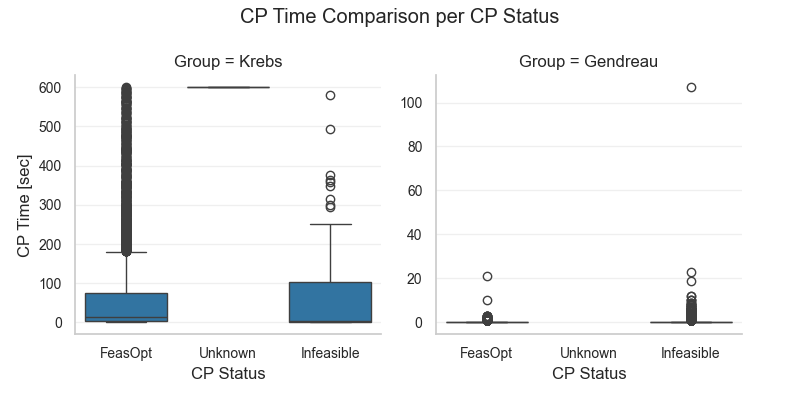
\includegraphics[width=\textwidth]{pictures/comparison_krebs_gendreau/boxplot_cp_time.png}
    \caption{Boxplot showing the different computation times for \krebsADataSetText and \gendreauDataSet.}
    \label{fig:comparison_krebs_gendreau_boxplot}
\end{figure}

The time average difference is caused by the group of routes labeled with \textit{Unknown} \gls{CP} status, which occurs, when
feasibility or infeasibility could not be proven in the maximum runtime of 600 seconds. From all routes from RD-1-1-1-10
33.6\% are classified as \textit{Unknown}. The distribution of \gls{LST} is shown in the following Figure~\ref{fig:comparison_krebs_gendreau_piechart}.

\begin{figure}[ht]
    \centering
    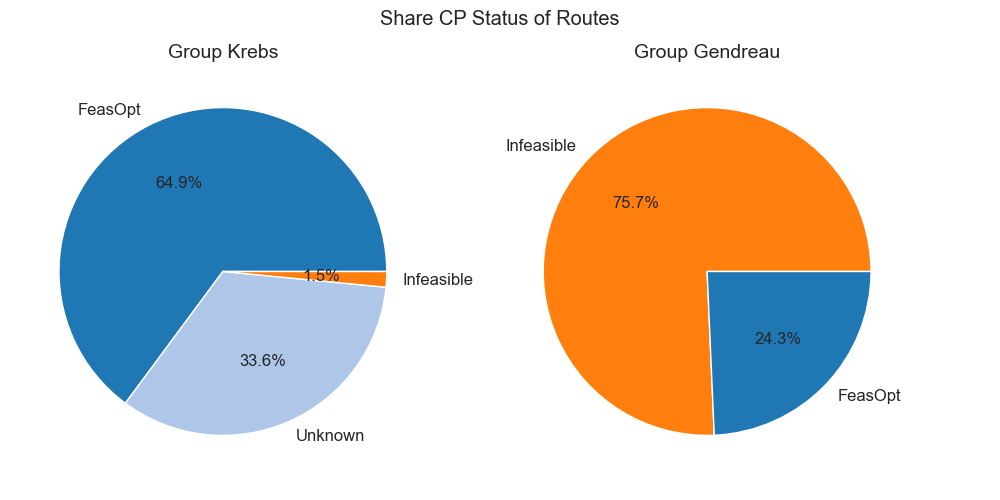
\includegraphics[width=\textwidth]{pictures/comparison_krebs_gendreau/pie_chart_share_cp_status.png}
    \caption{Big share of unknown labeled tours for the \krebsADataSet.}
    \label{fig:comparison_krebs_gendreau_piechart}
\end{figure}
All routes classified as \textit{Unknown} will be considered as \textit{Infeasible}, as outlined in Section~\ref{sec:DataRetrieval}. But
as the true label is not used, the model performance is weakened as possibly feasible routes will be labeled as infeasible. The
next Figure~\ref{fig:comparison_krebs_gendreau_numberItems} shows the effect of the number of items to the \gls{CP} time and the status.

\begin{figure}[ht]
    \centering
    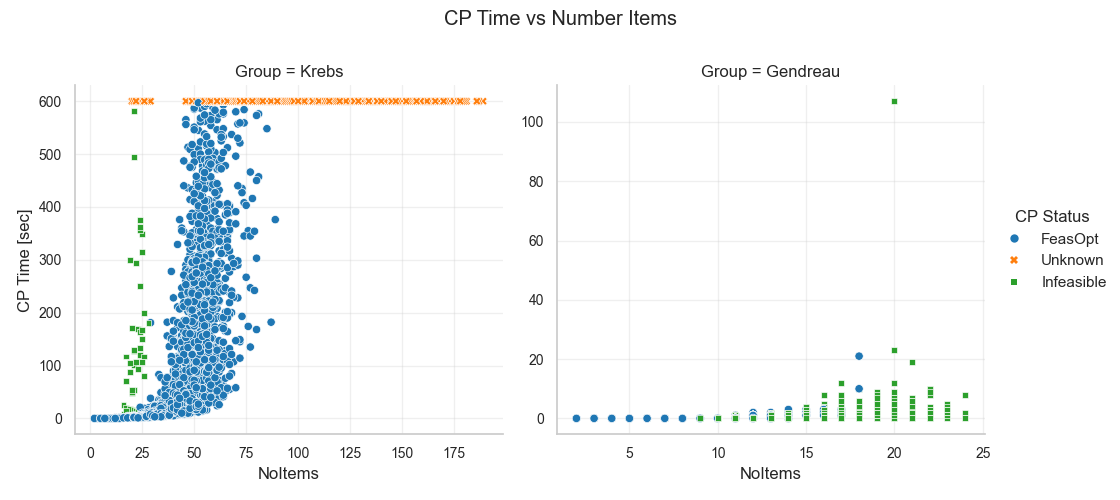
\includegraphics[width=0.9\textwidth]{pictures/comparison_krebs_gendreau/number_items_cp_status.png}
    \caption{Influence of number of items on the computational time.}
    \label{fig:comparison_krebs_gendreau_numberItems}
\end{figure}

The computation time literally explodes when more than 50 items are considered in a route, leading to an \textit{Unknown} \gls{CP} status, and
infeasible labels in the train dataset. So in the end, new long routes which improve the solution quality will always be classified as infeasible
and the exact computation time with the \gls{CP} solver takes too long to be used in a heuristic. As fewer items are considered in the dataset
RD-2-30-20-10 the \gls{CP} time increases only minimal, when the maximum number of 25 items is reached.

\subsection{Save strategy}
\label{subsec:challenges_krebs_save}

The results obtained by the B\&C algorithm from \cite{tamke_branch-and-cut_2024} are with an average gap of 3.14\% pretty good. However, some limitations
of the branch-and-cut algorithm caused issues solving instances from \krebsADataSetText. As shown before, the labeling of one route takes approximately
1000 times longer than for the \gendreauDataSetText, causing the dilemma, if either the time limit for the \gls{CP} solver within the B\%C solver
must be limited causing a lot of \textit{Unknown} and \textit{Invalid} labeled tours and the interrupting of the B\%C solver or choosing
a high time limit, which restricts the B\%C solver in testing many solutions as the feasibility check is time intensive. The first option
was chosen and the B\%C was modified to avert some interruptions, but not all. Therefore some runs creating the train datasets are labeled with
B and C in Table~\ref{tab:bc_results_krebs}. The obtained datasets of the save strategy are shown in Table~\ref{tab:saved_instances_krebs}
and the most suiting dataframe can already be identified by looking at the datasets characteristics. The number of routes with two customers
are dominating the total number of routes, if the datasets are not shrinked or trimmed, as can be seen in Figure~\ref{fig:route-dists_save_krebs}. Furthermore, the average relative mass and volume and
is very low due to the imbalance of the route length.

\begin{figure}[ht]
    \centering
    \begin{subfigure}[t]{.5\textwidth}
        \centering
        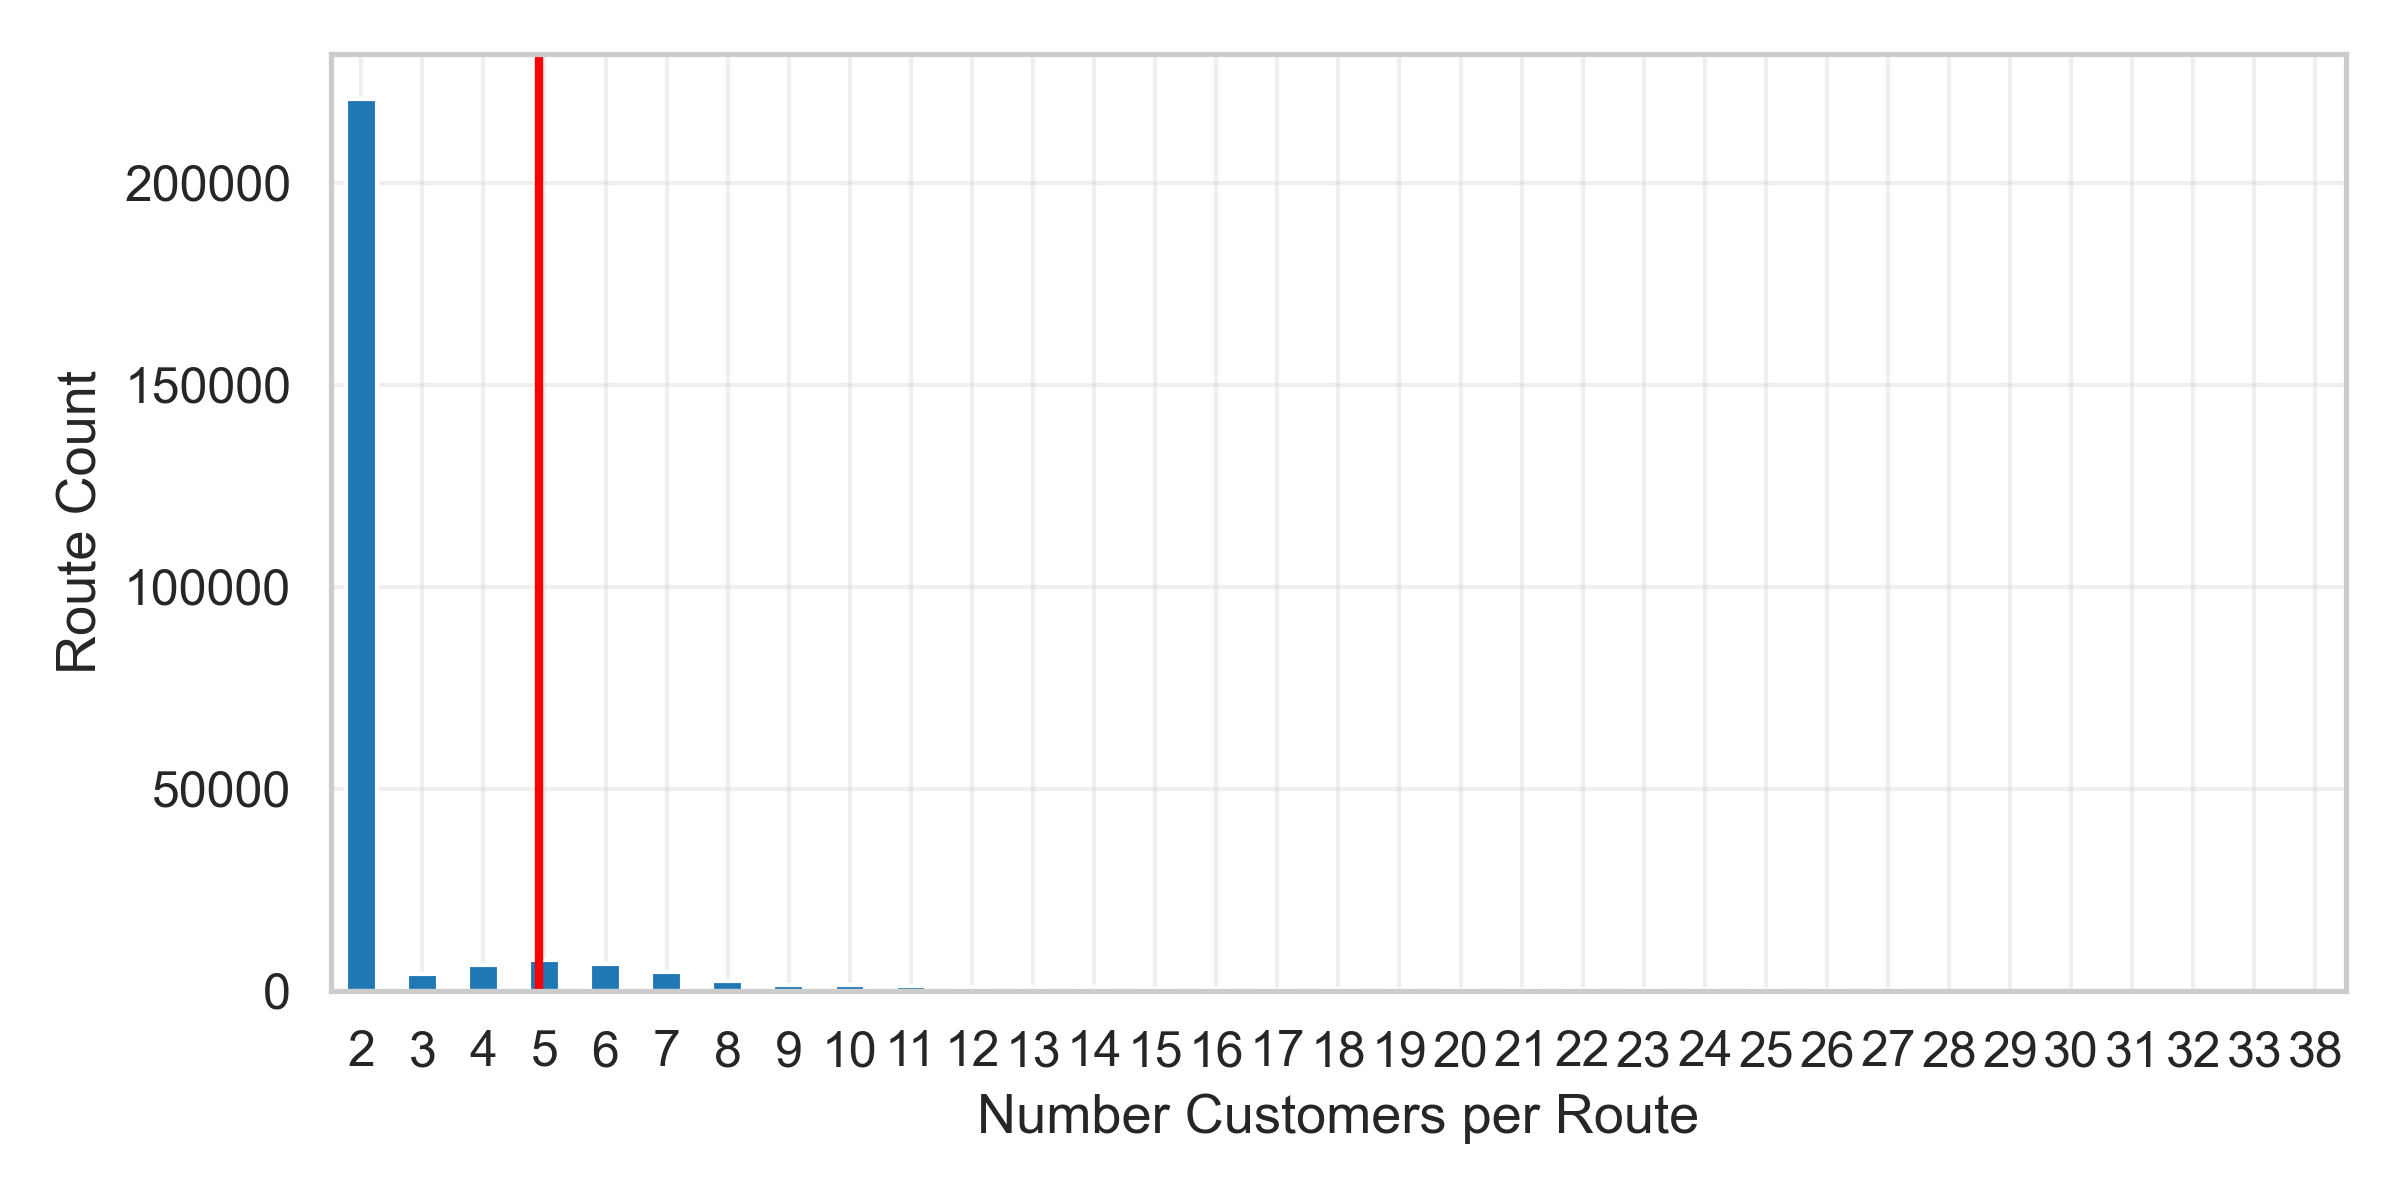
\includegraphics[width=\linewidth]{pictures/dataset_structure/no_cust_plot_krebs_28880_600_WS.png}
        \caption{Dataset KS-Complete-WS}
        \label{fig:ds-a-krebs}
    \end{subfigure}%
    \begin{subfigure}[t]{.5\textwidth}
        \centering
        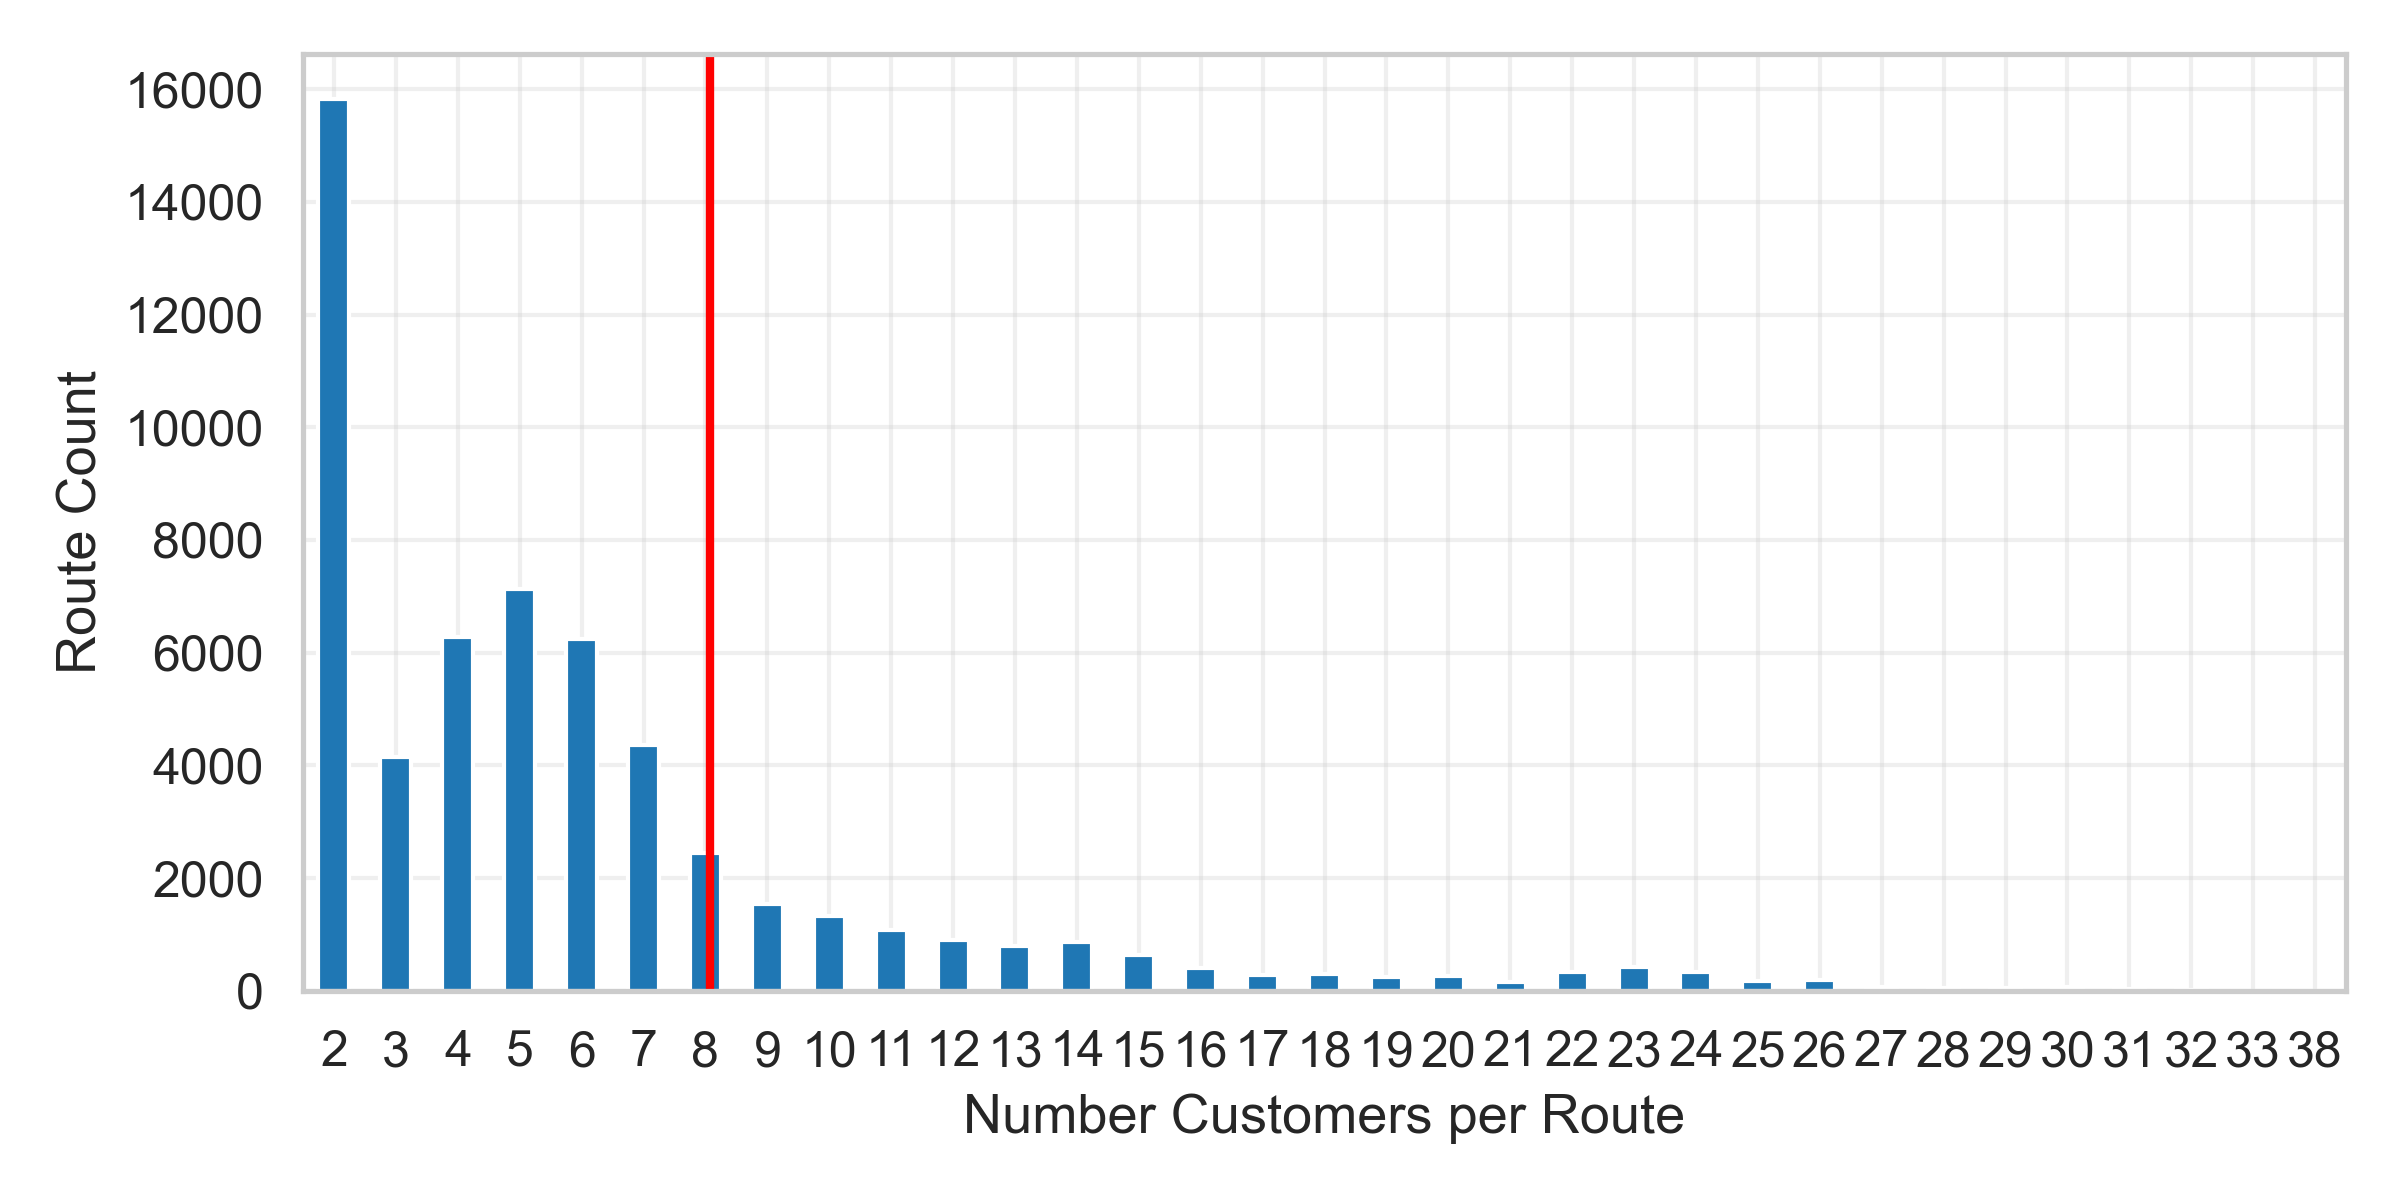
\includegraphics[width=\linewidth]{pictures/dataset_structure/no_cust_plot_krebs_28880_600_WS_shrinked094.png}
        \caption{Dataset KS-Shrinked-WS}
        \label{fig:ds-b-krebs}
    \end{subfigure}
    \caption{Distribution of route length for the two adapted save strategy datasets. The red vertical line represents the average
        number of customers.}
    \label{fig:route-dists_save_krebs}
\end{figure}

The prevaillance of routes with 2 customers is also shown in the following Figure~\ref{fig:route-feasibility_save_krebs}, displaying the number of routes found per instance and
the balance of feasible and infeasible routes. The number of found routes is dropping by 205.027 routes in total, and therefore
also the prevailing share of feasible routes with 2 customers.

\begin{figure}[ht]
    \centering
    \begin{subfigure}[t]{.5\textwidth}
        \centering
        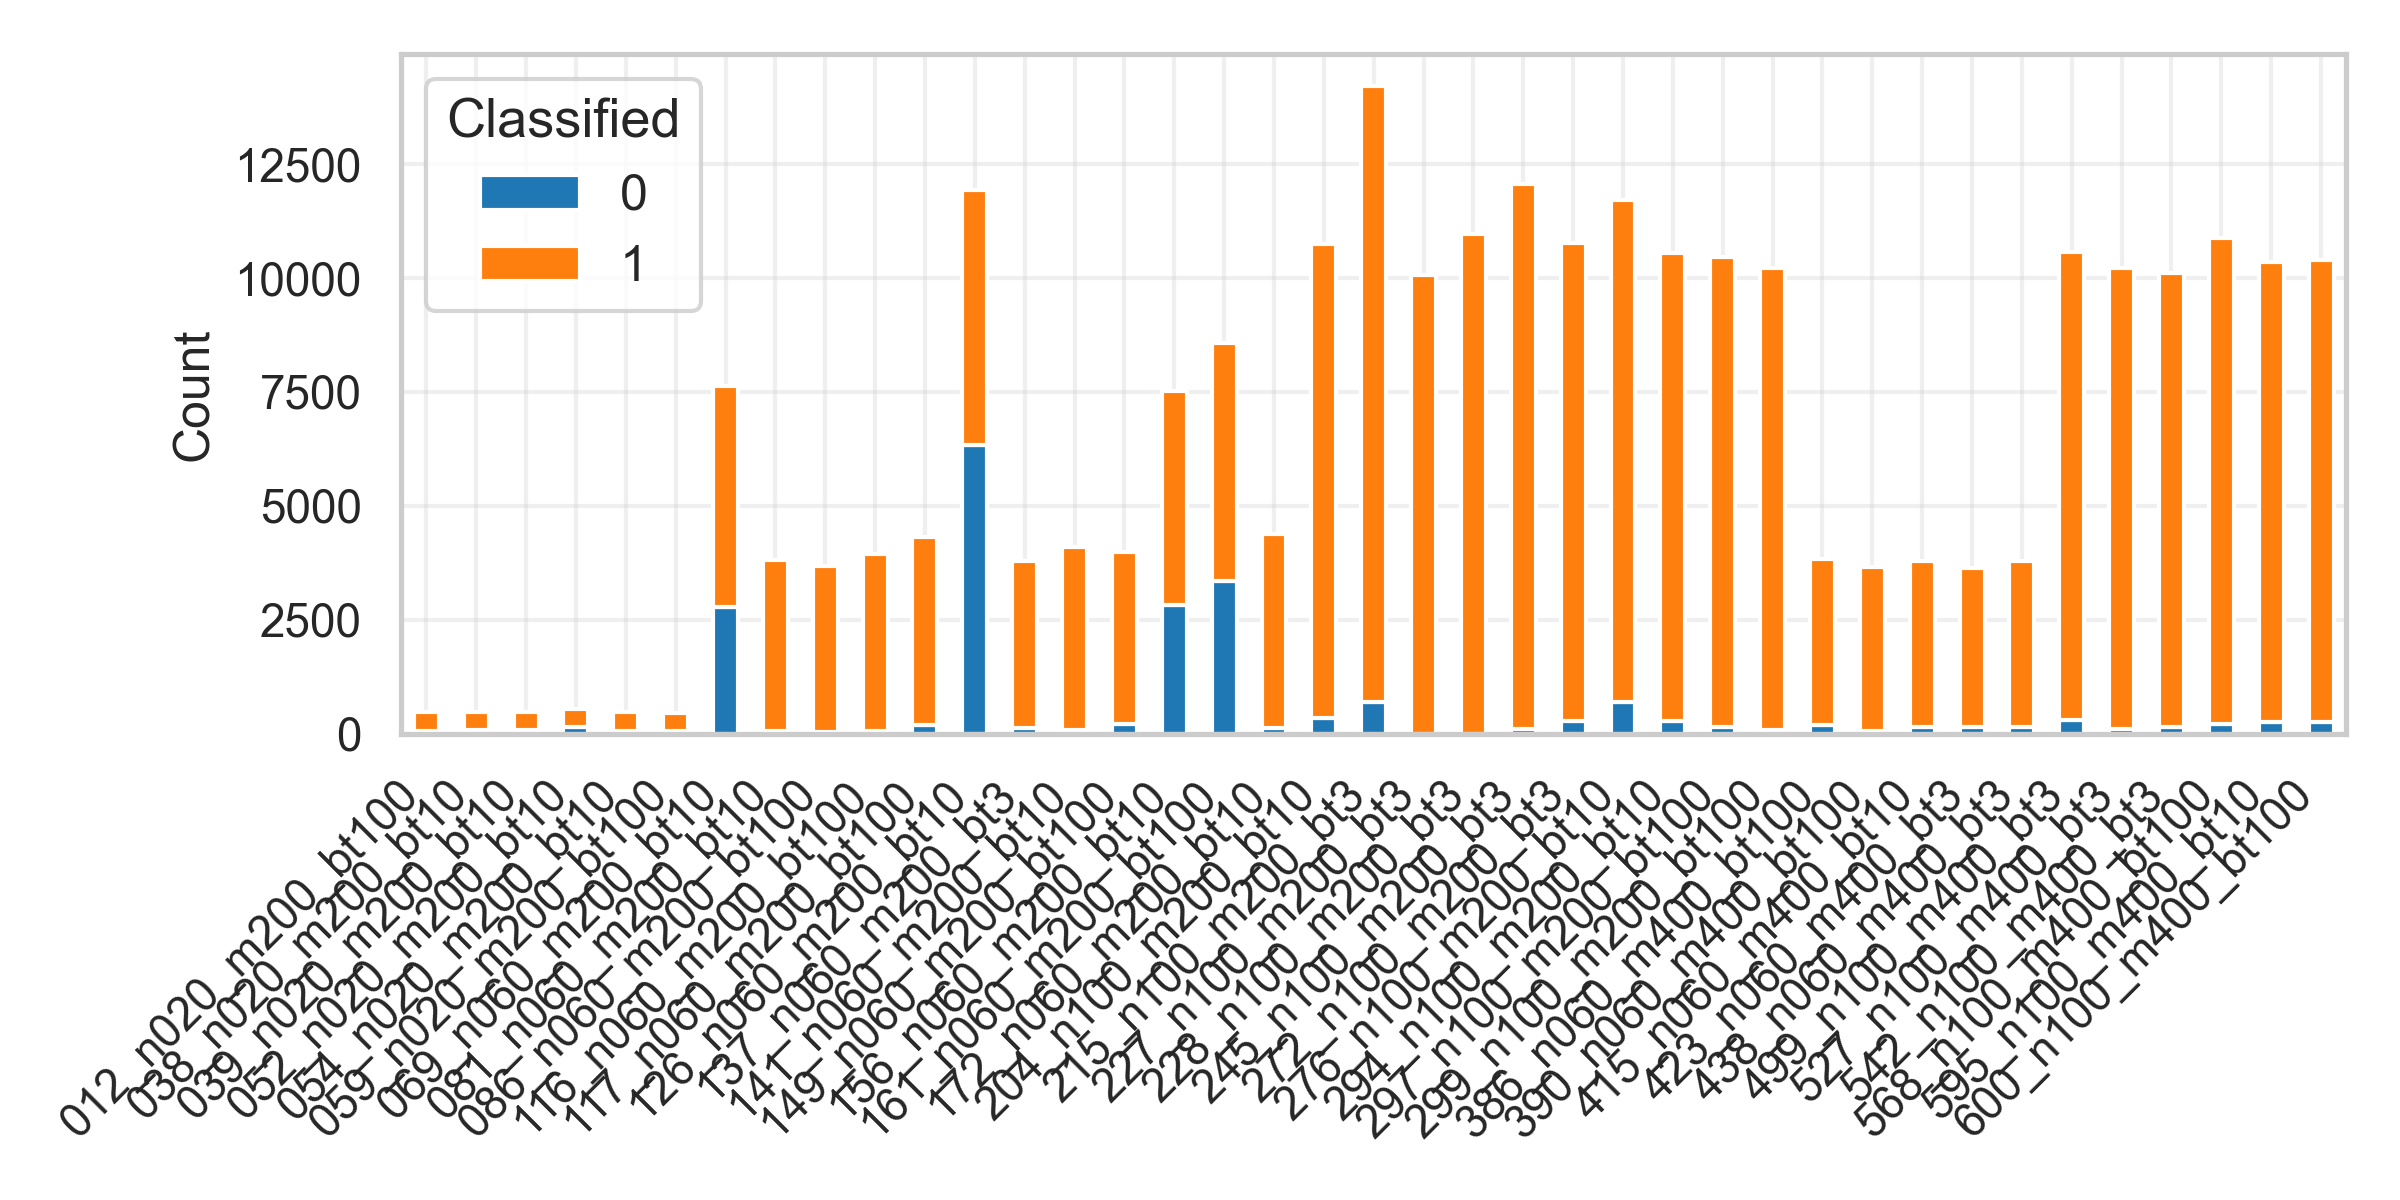
\includegraphics[width=\linewidth]{pictures/dataset_structure/distribution_plot_krebs_28880_600_WS.png}
        \caption{Dataset KS-Complete-WS}
        \label{fig:ds-a-krebs_x}
    \end{subfigure}%
    \begin{subfigure}[t]{.5\textwidth}
        \centering
        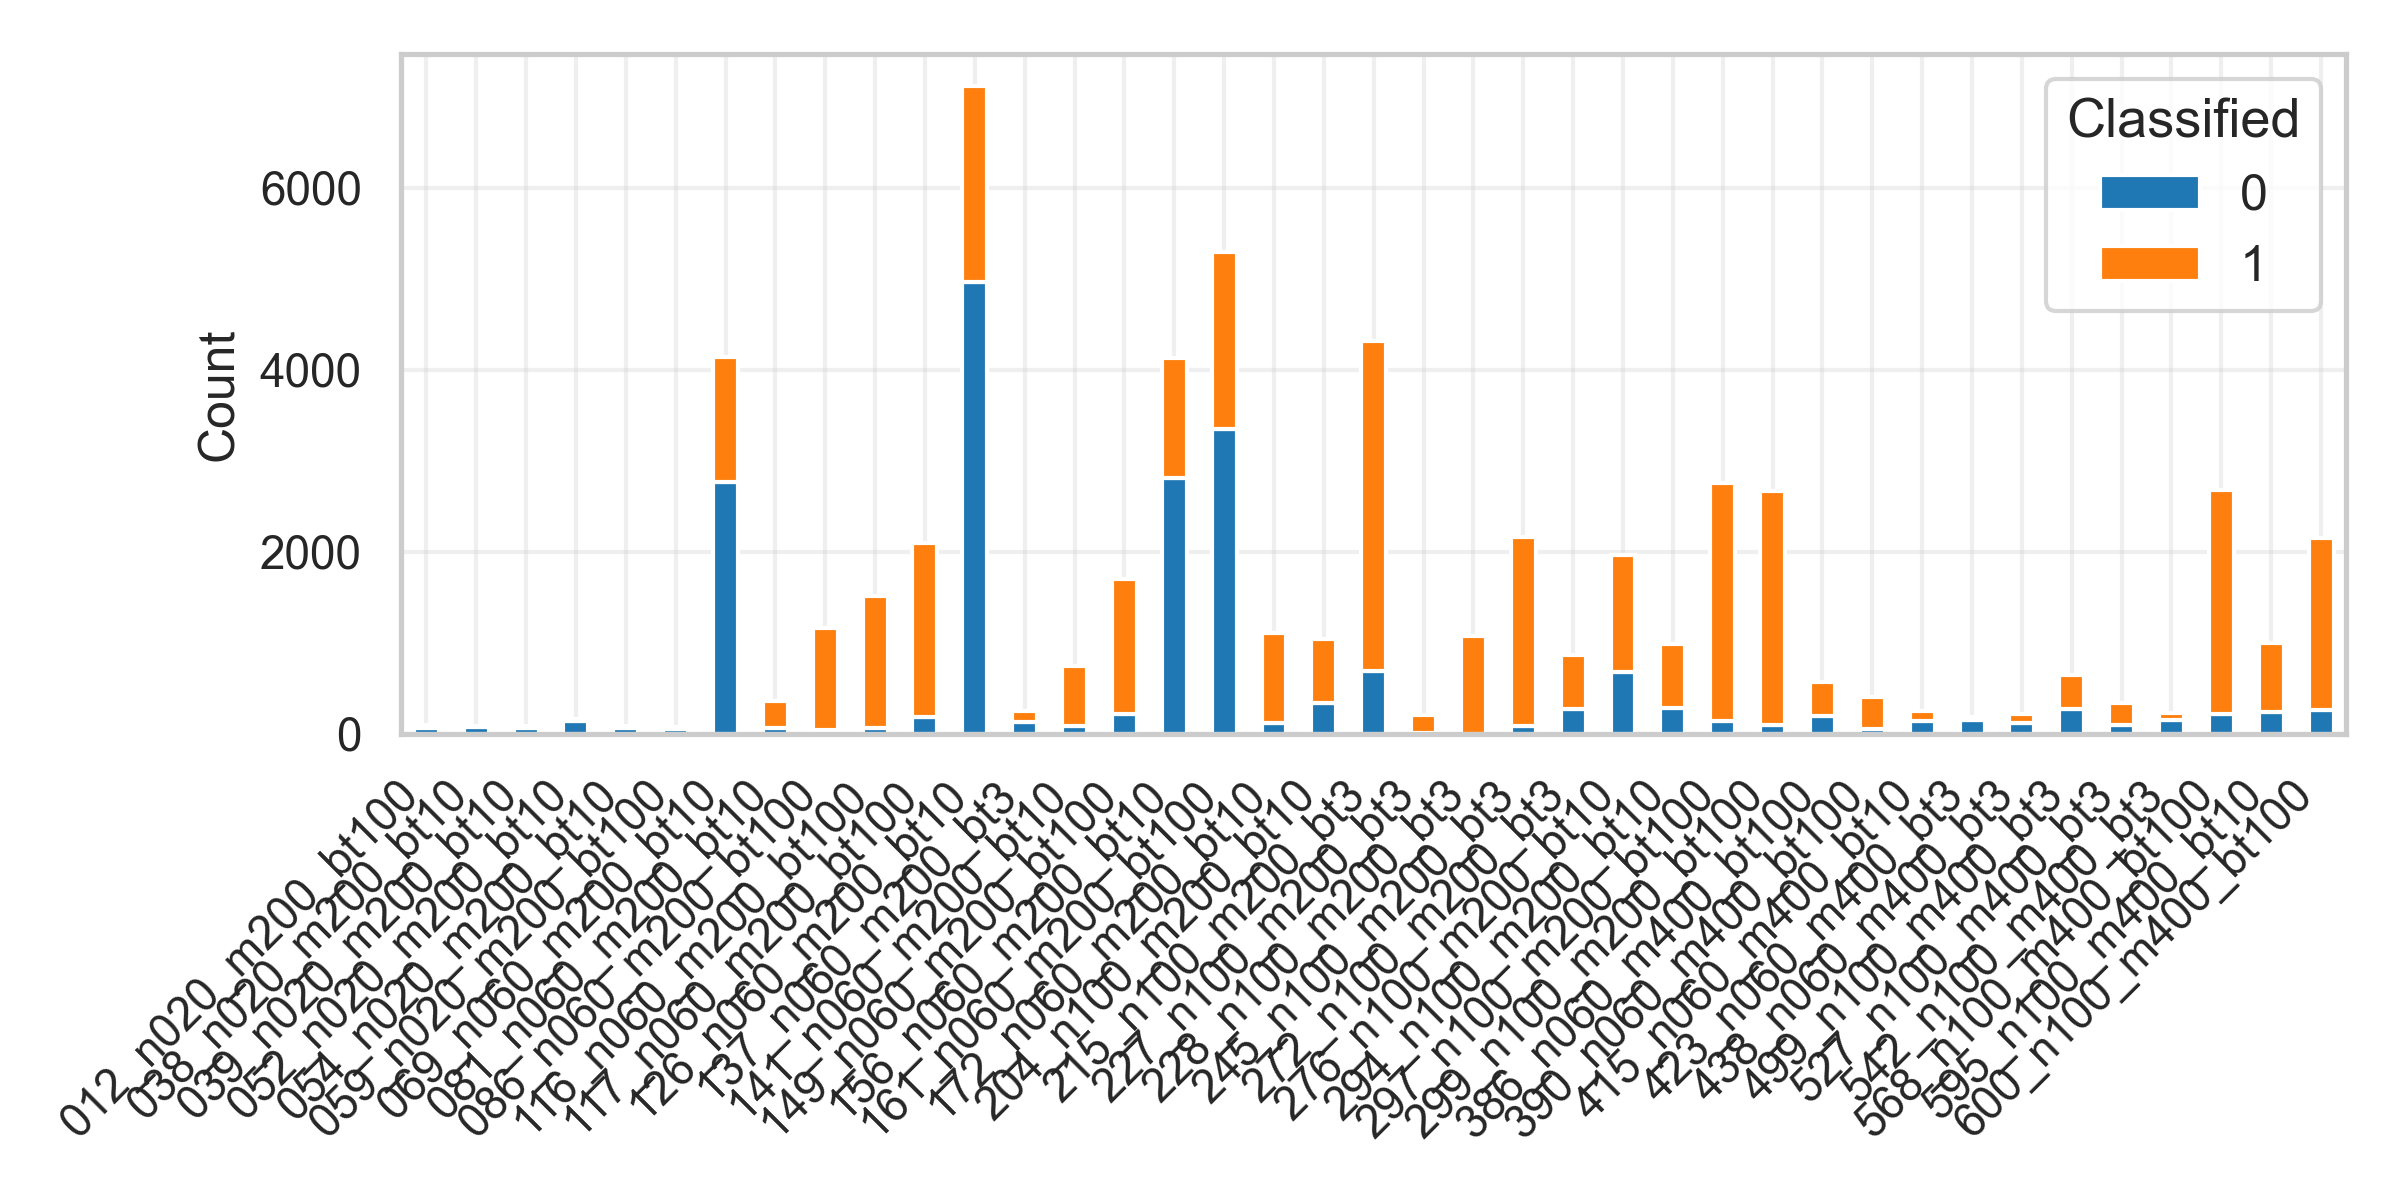
\includegraphics[width=\linewidth]{pictures/dataset_structure/distribution_plot_krebs_28880_600_WS_shrinked094.png}
        \caption{Dataset KS-Shrinked-WS}
        \label{fig:ds-b-krebs_l}
    \end{subfigure}
    \caption{Distribution of route length for the two adapted save strategy datasets. The red vertical line represents the average
        number of customers.}
    \label{fig:route-feasibility_save_krebs}
\end{figure}

The trimmed dataset will not be used further, as this datasets lacks the data to predict feasible routes with two customers as only
infeasible tours for this route length are present in the dataset.

\begin{table}[ht]
    \centering
    \begin{tabular}{l c c c c c c }
        \toprule
        Name           & Sets                 & Routes & Routes Len = 2 & Balance   & Rel. Vol & Rel. Mass \\
        \midrule
        KS-Complete-WS & \multirow{3}{*}{Yes} & 261989 & 220860         & 92.4/7.6  & 0.18     & 0.20      \\
        KS-Trimmed-WS  &                      & 41337  & 208            & 52.1/47.9 & 0.58     & 0.63      \\
        KS-Shrinked-WS &                      & 56962  & 15833          & 65.3/34.7 & 0.43     & 0.48      \\        \midrule
        KS-Complete    & \multirow{3}{*}{No}  & 256786 & 220860         & 94.3/5.7  & 0.16     & 0.19      \\
        KS-Trimmed     &                      & 36134  & 208            & 59.6/40.4 & 0.54     & 0.61      \\
        KS-Shrinked    &                      & 51759  & 15833          & 71.8/28.2 & 0.39     & 0.46      \\

        \bottomrule
    \end{tabular}
    \caption{Save strategy train datsets from \krebsADataSet.}
    \label{tab:saved_instances_krebs}
\end{table}